\chapter{Measuring Teacher Quality}

\fancyhead[L]{ECON0024}
\fancyhead[C]{Ch.9 Measuring Teacher Quality}
\fancyhead[R]{Xiaotian Tian}
\fancyfoot[L]{\hyperlink{tableofcontents}{Back to Table of Contents}}
\fancyfoot[R]{Xiaotian Tian}

\section{Empirical Facts: Increasing Educational Spending and Stagnant Outcome}

    \subsection{Increasing Educational Spending}
        
        \subsubsection{Educational Spending in U.S.}
            \begin{figure}[H]
                \centering
                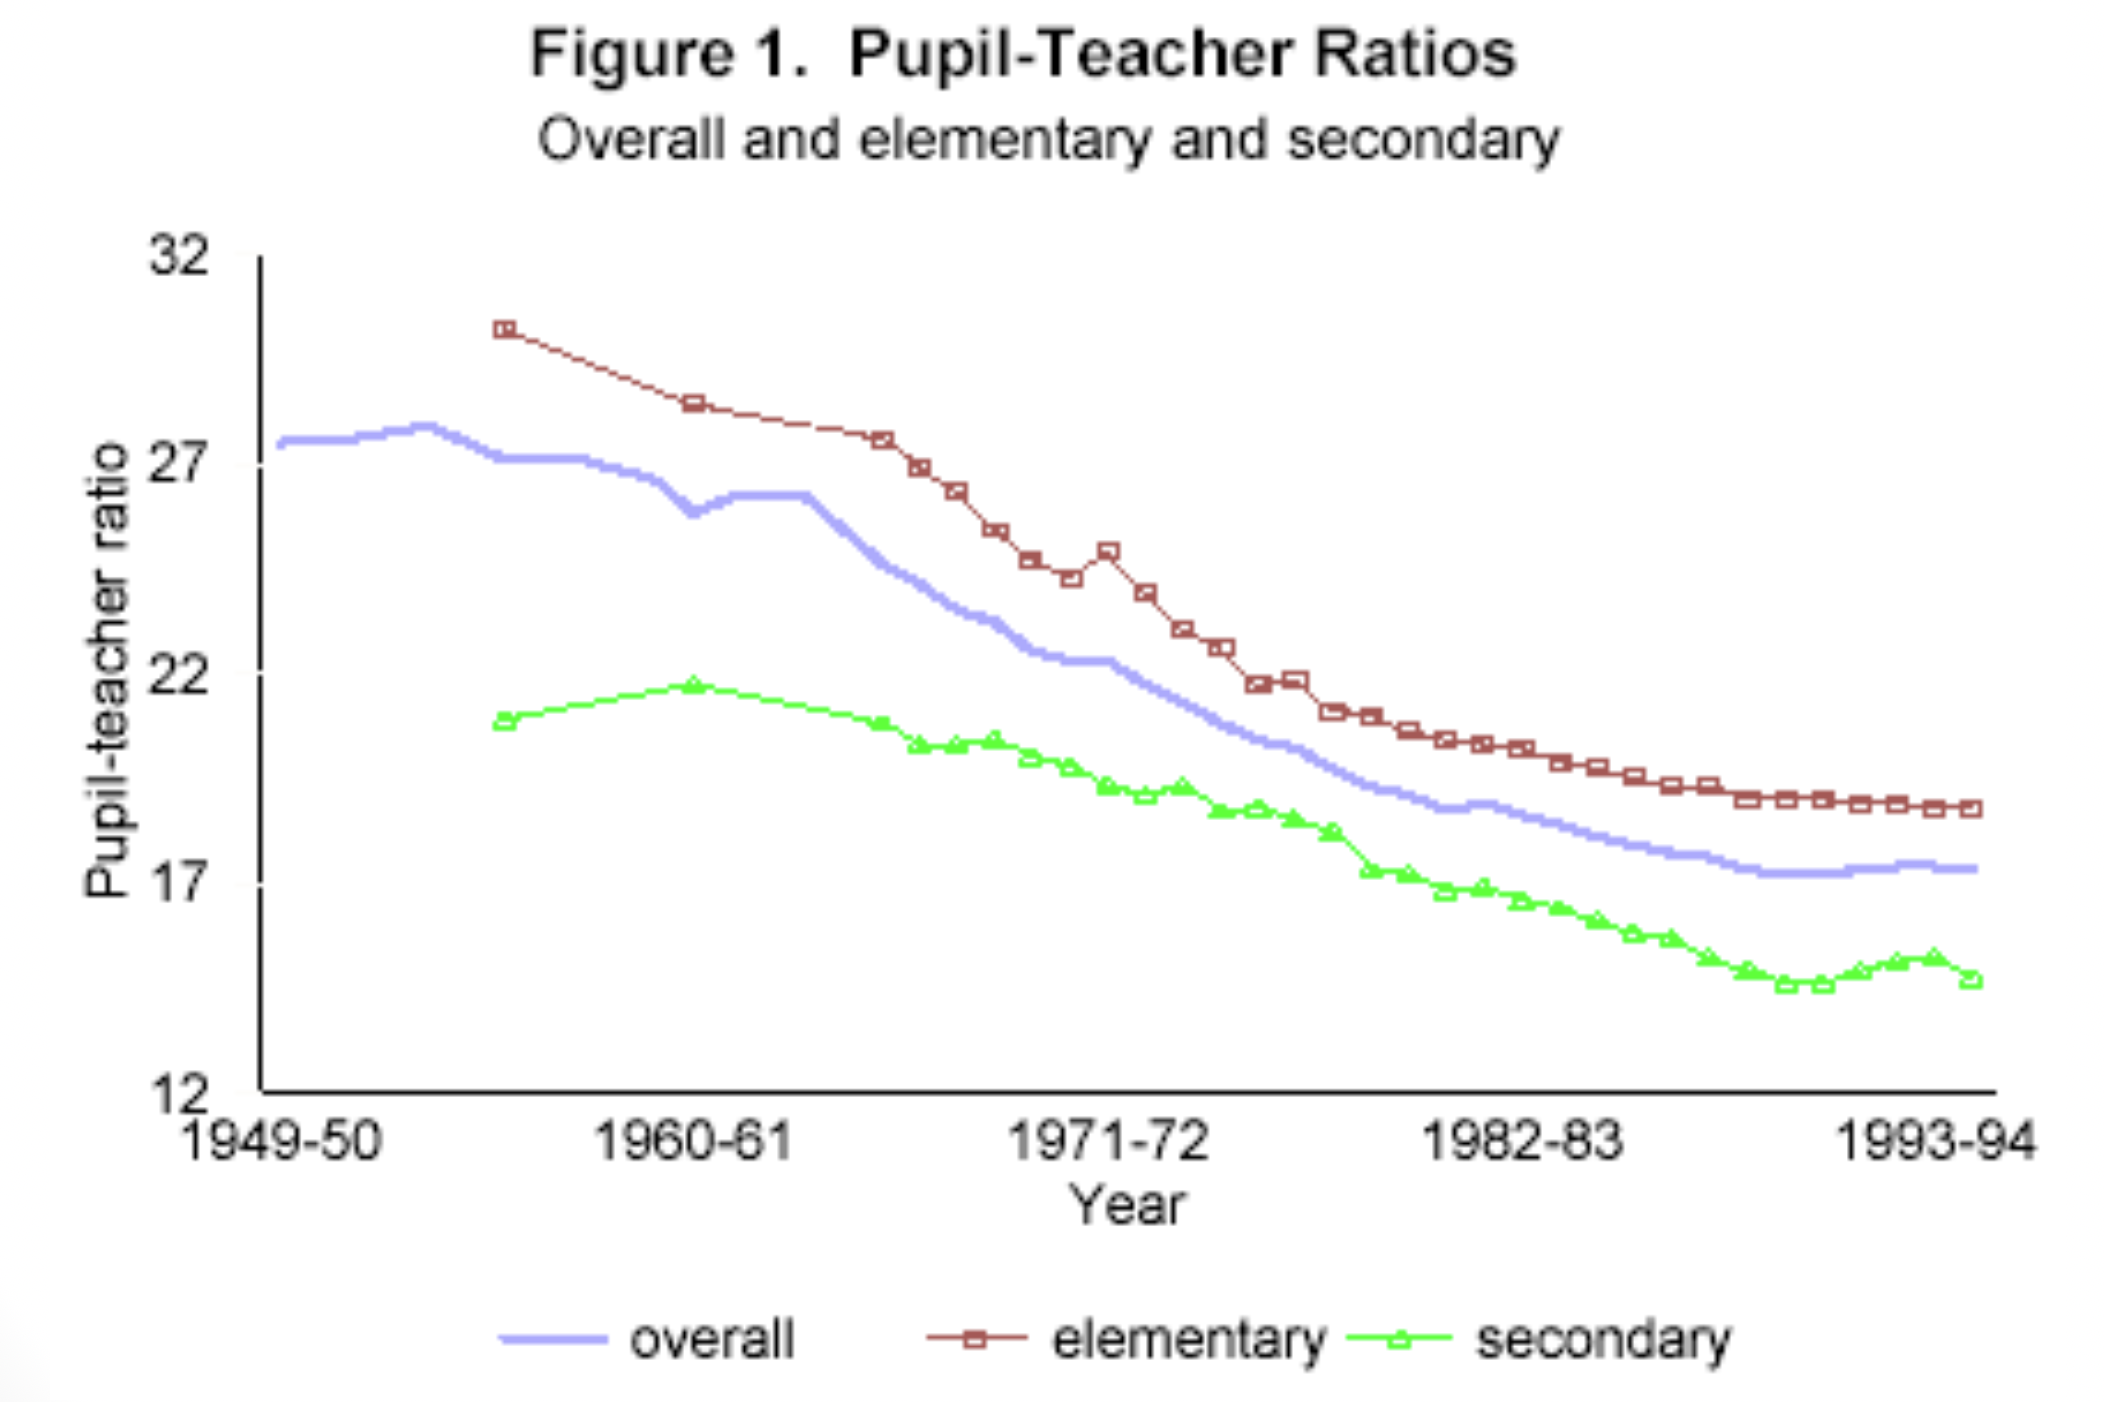
\includegraphics[width=4in]{images/ch9/9 us res 1.png}
                \caption{U.S. Pupil-Teacher Ratios (\cite{hanushek_handbook_2016})}
            \end{figure}
            \begin{figure}[H]
                \centering
                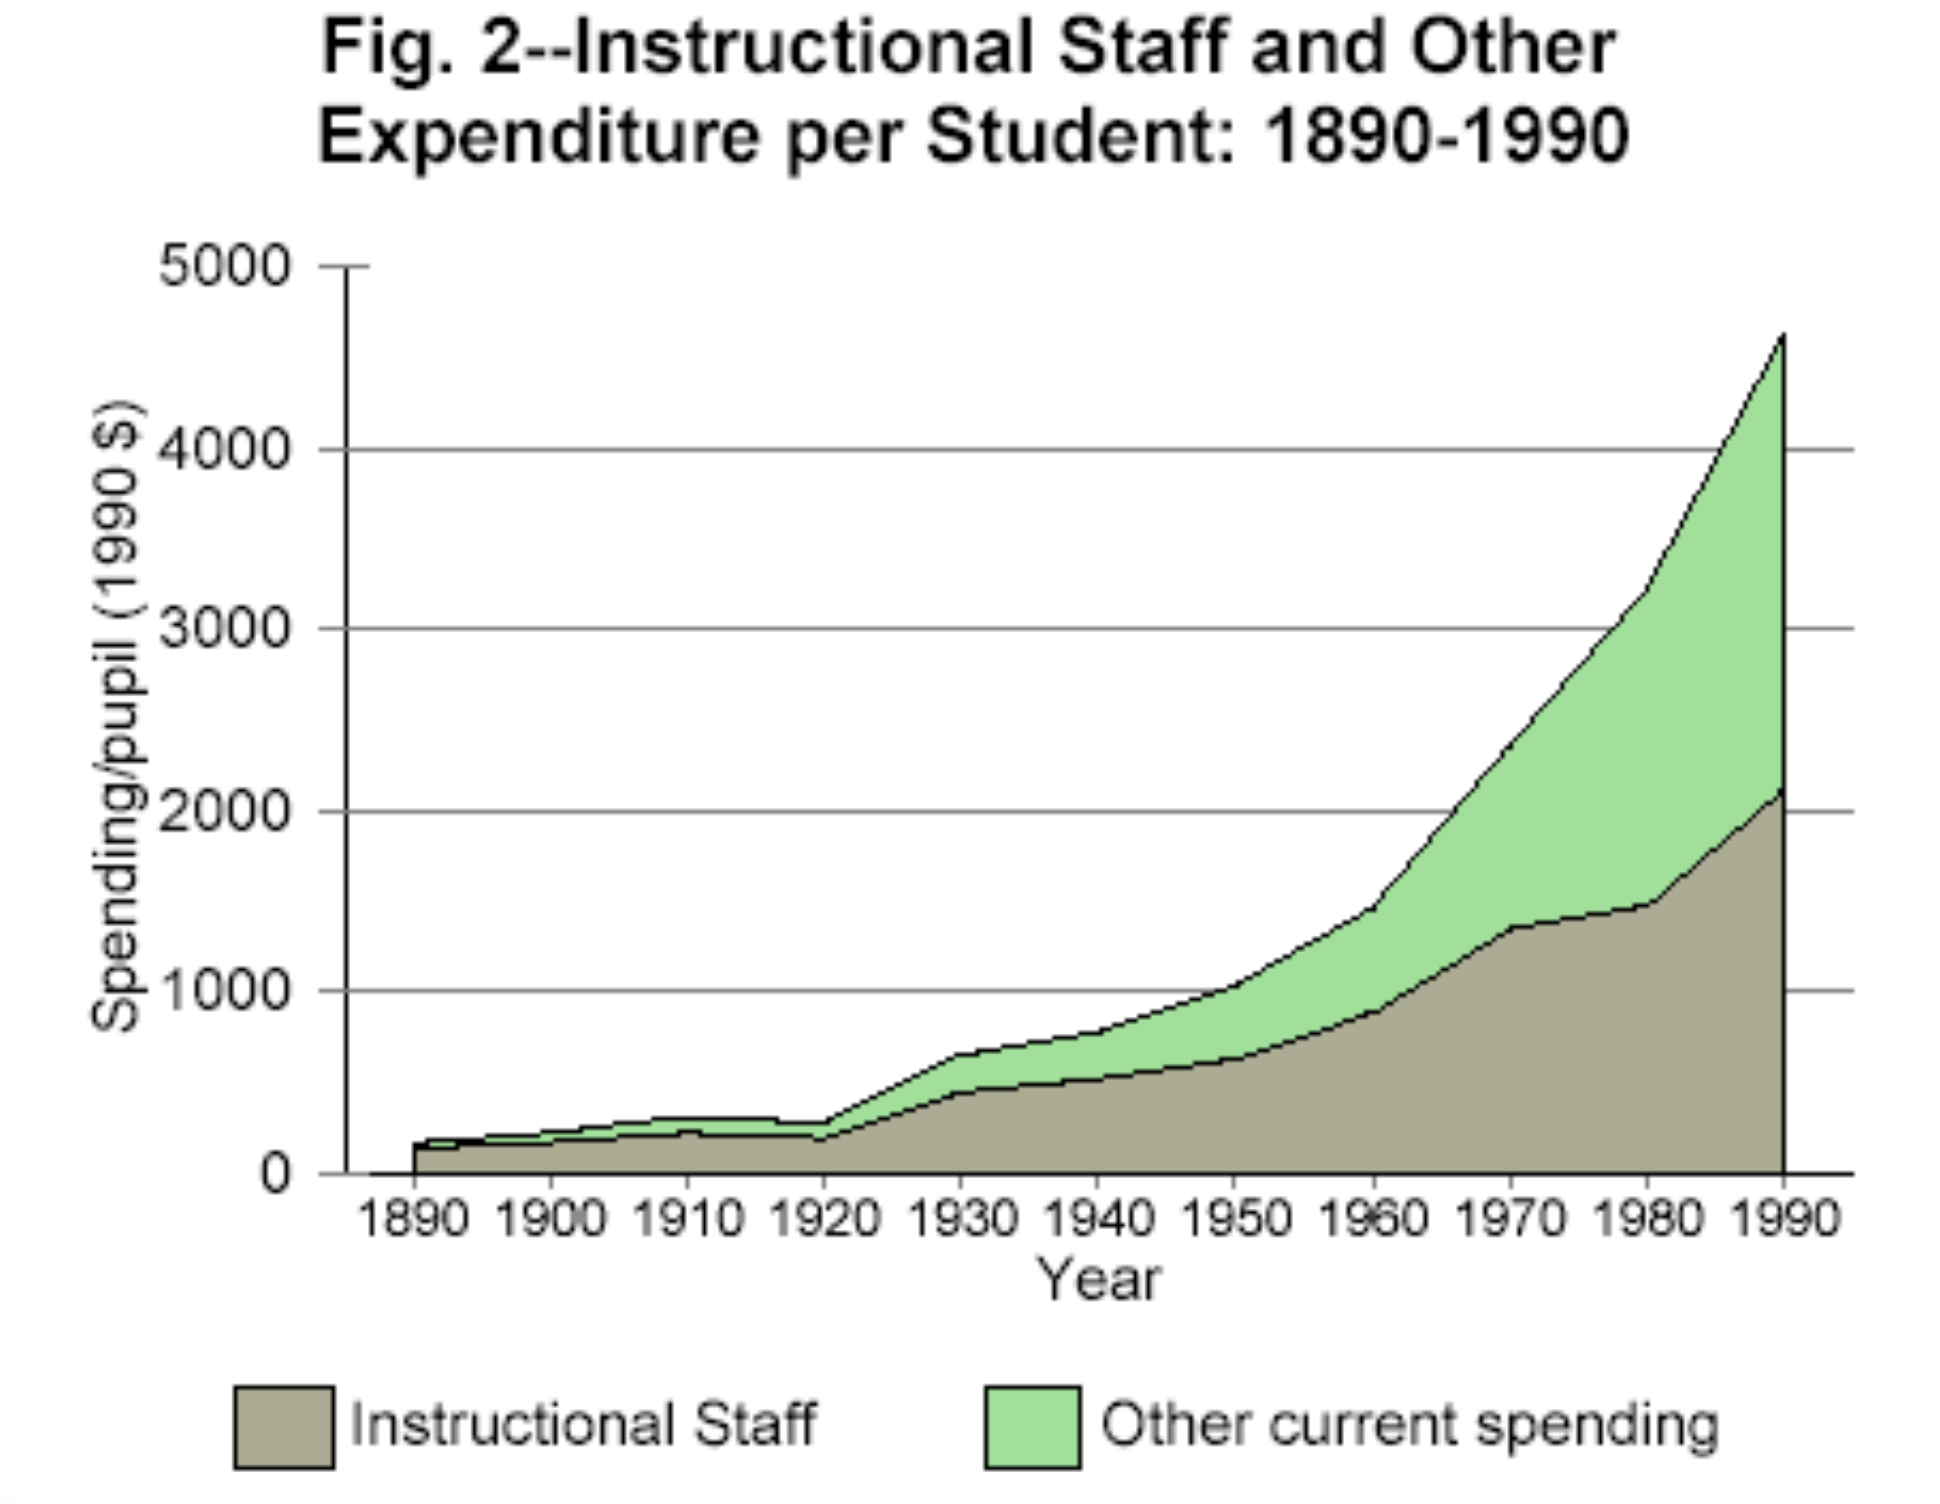
\includegraphics[width=4in]{images/ch9/9 us res 2.png}
                \caption{U.S. Instructional Staff and Other Expenditure per Student: 1890-1990 (\cite{hanushek_handbook_2016})}
            \end{figure}
            In U.S., more resources have been allocated to education: the pupil-teacher ratios declined, and the expenditure per student increased.
            
        \subsubsection{Educational Spending in the UK}
            \begin{figure}[H]
                \centering
                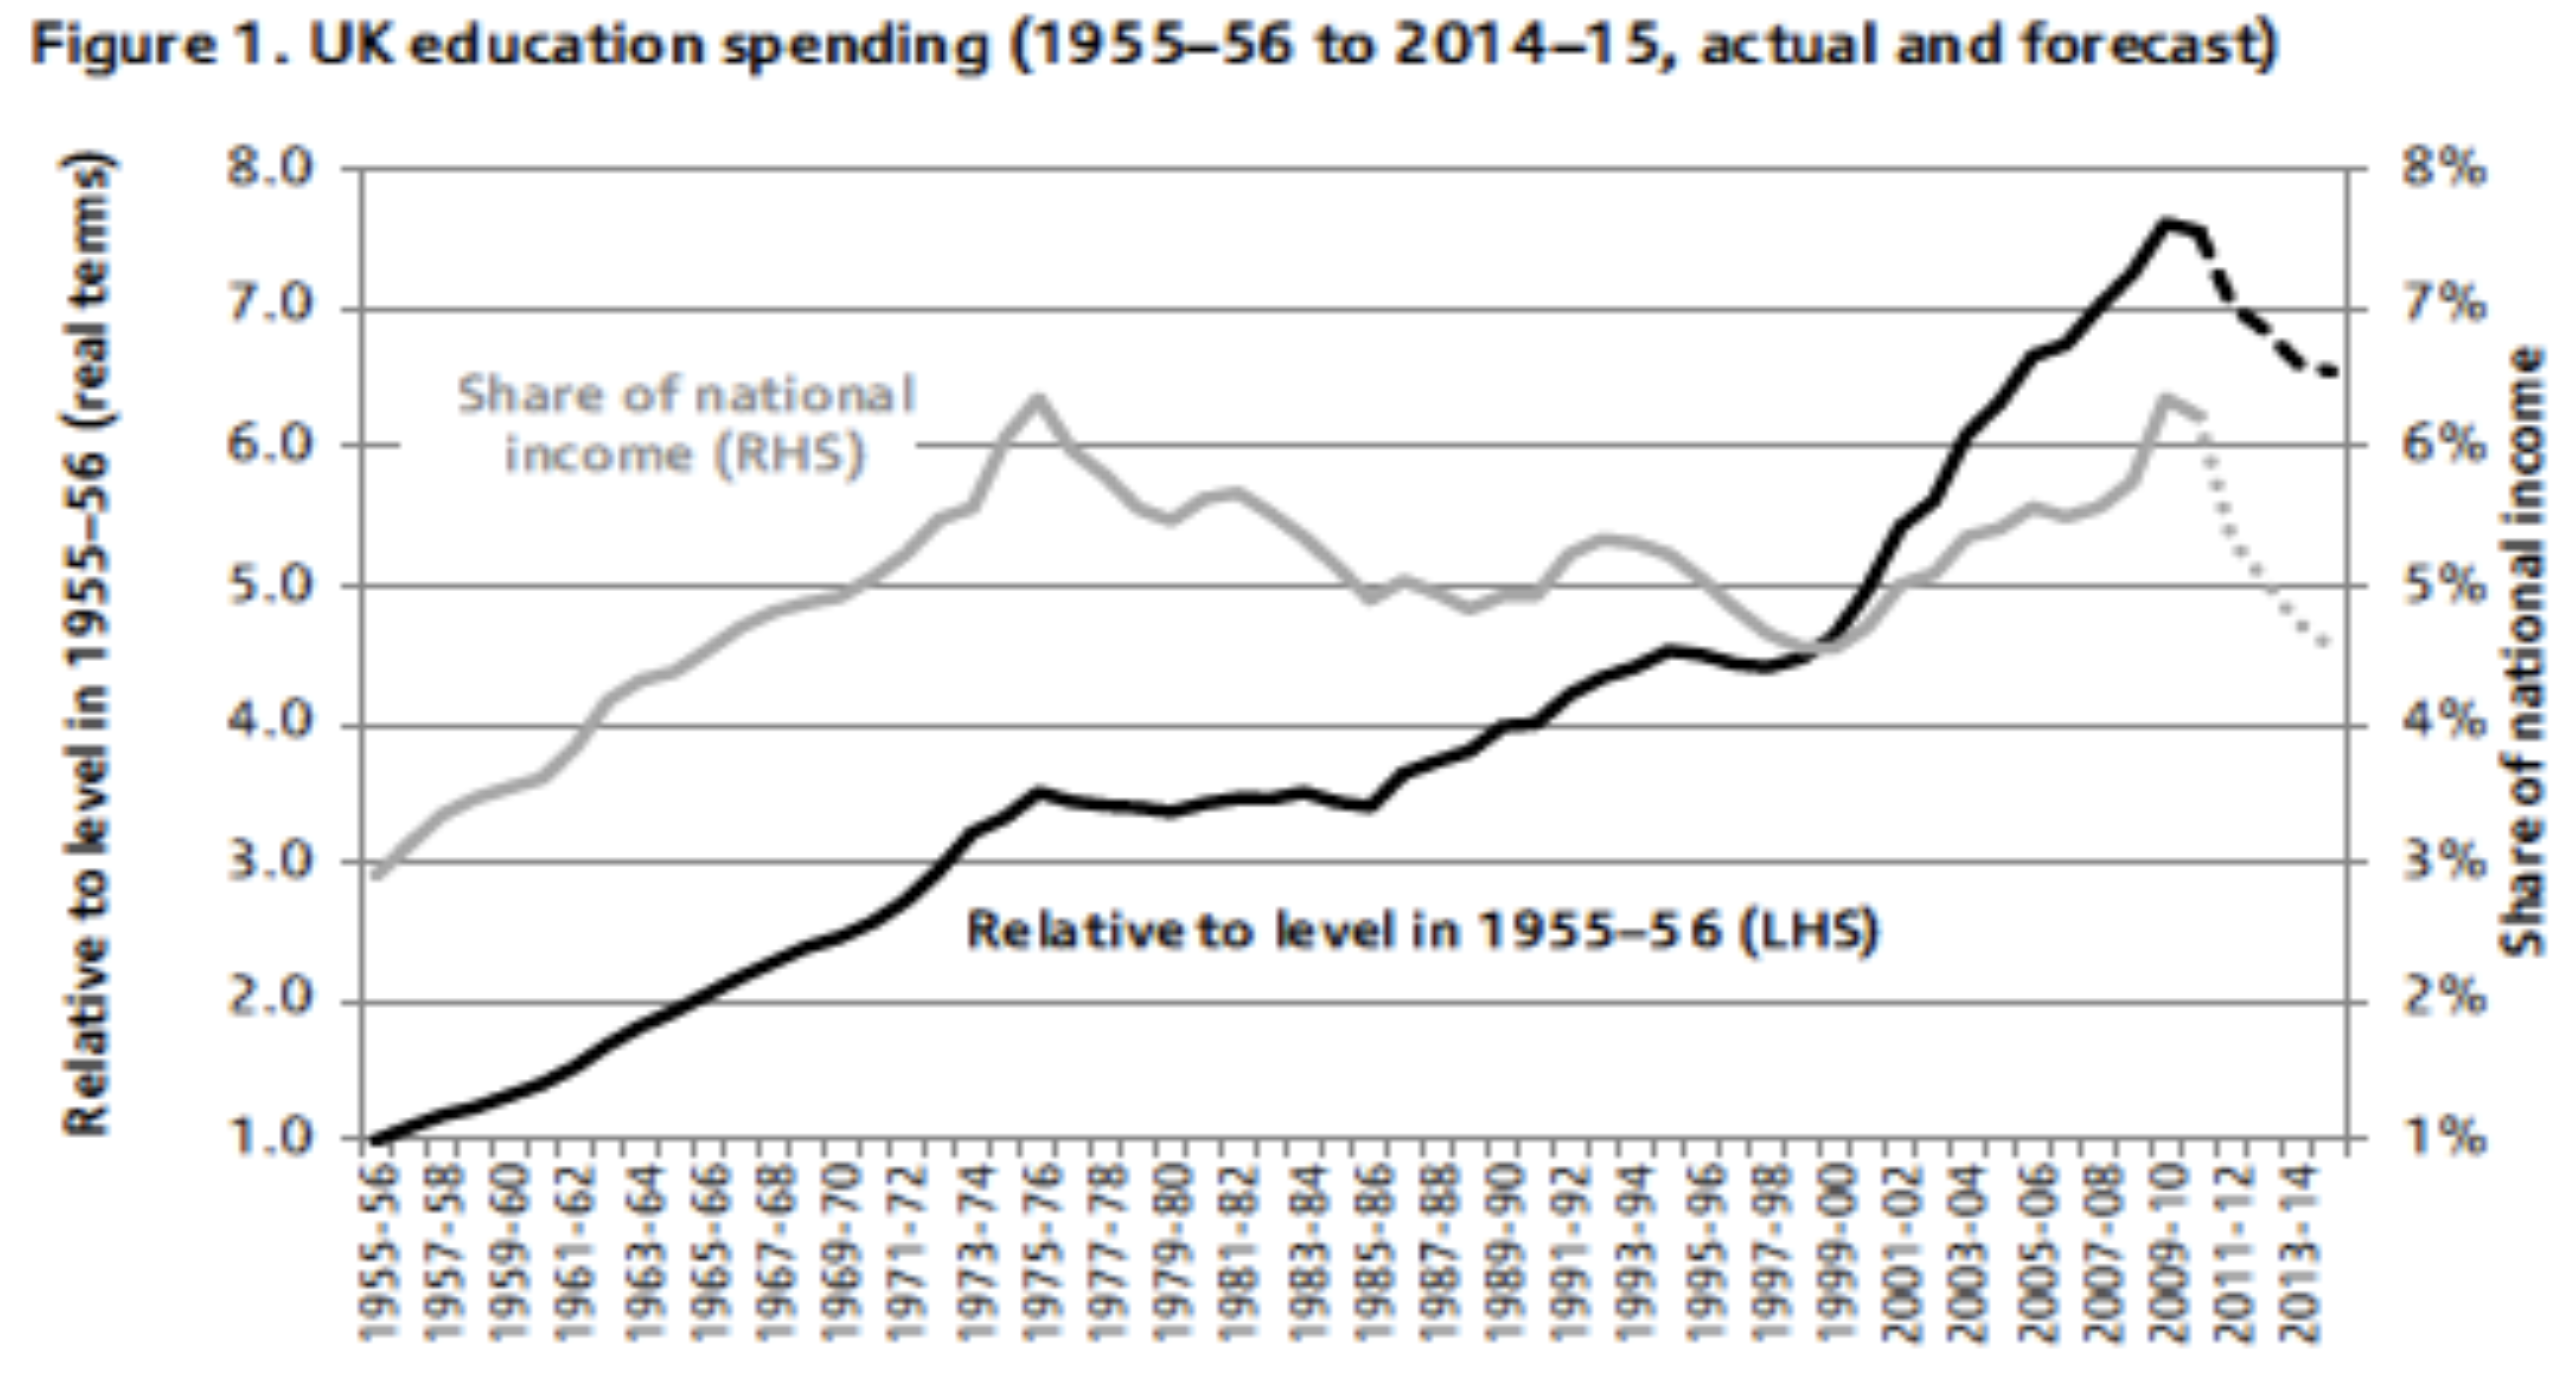
\includegraphics[width=4in]{images/ch9/9 uk res 1.png}
                \caption{UK Education Spending (1955/6-2014/5)}
            \end{figure}
            The absolute level of education spending in the UK also kept increasing, though its share of national income levelled off.
            
    
    \subsection{Stagnant Outcome}
        
        \subsubsection{School Results in U.S.}
            \begin{figure}[H]
                \centering
                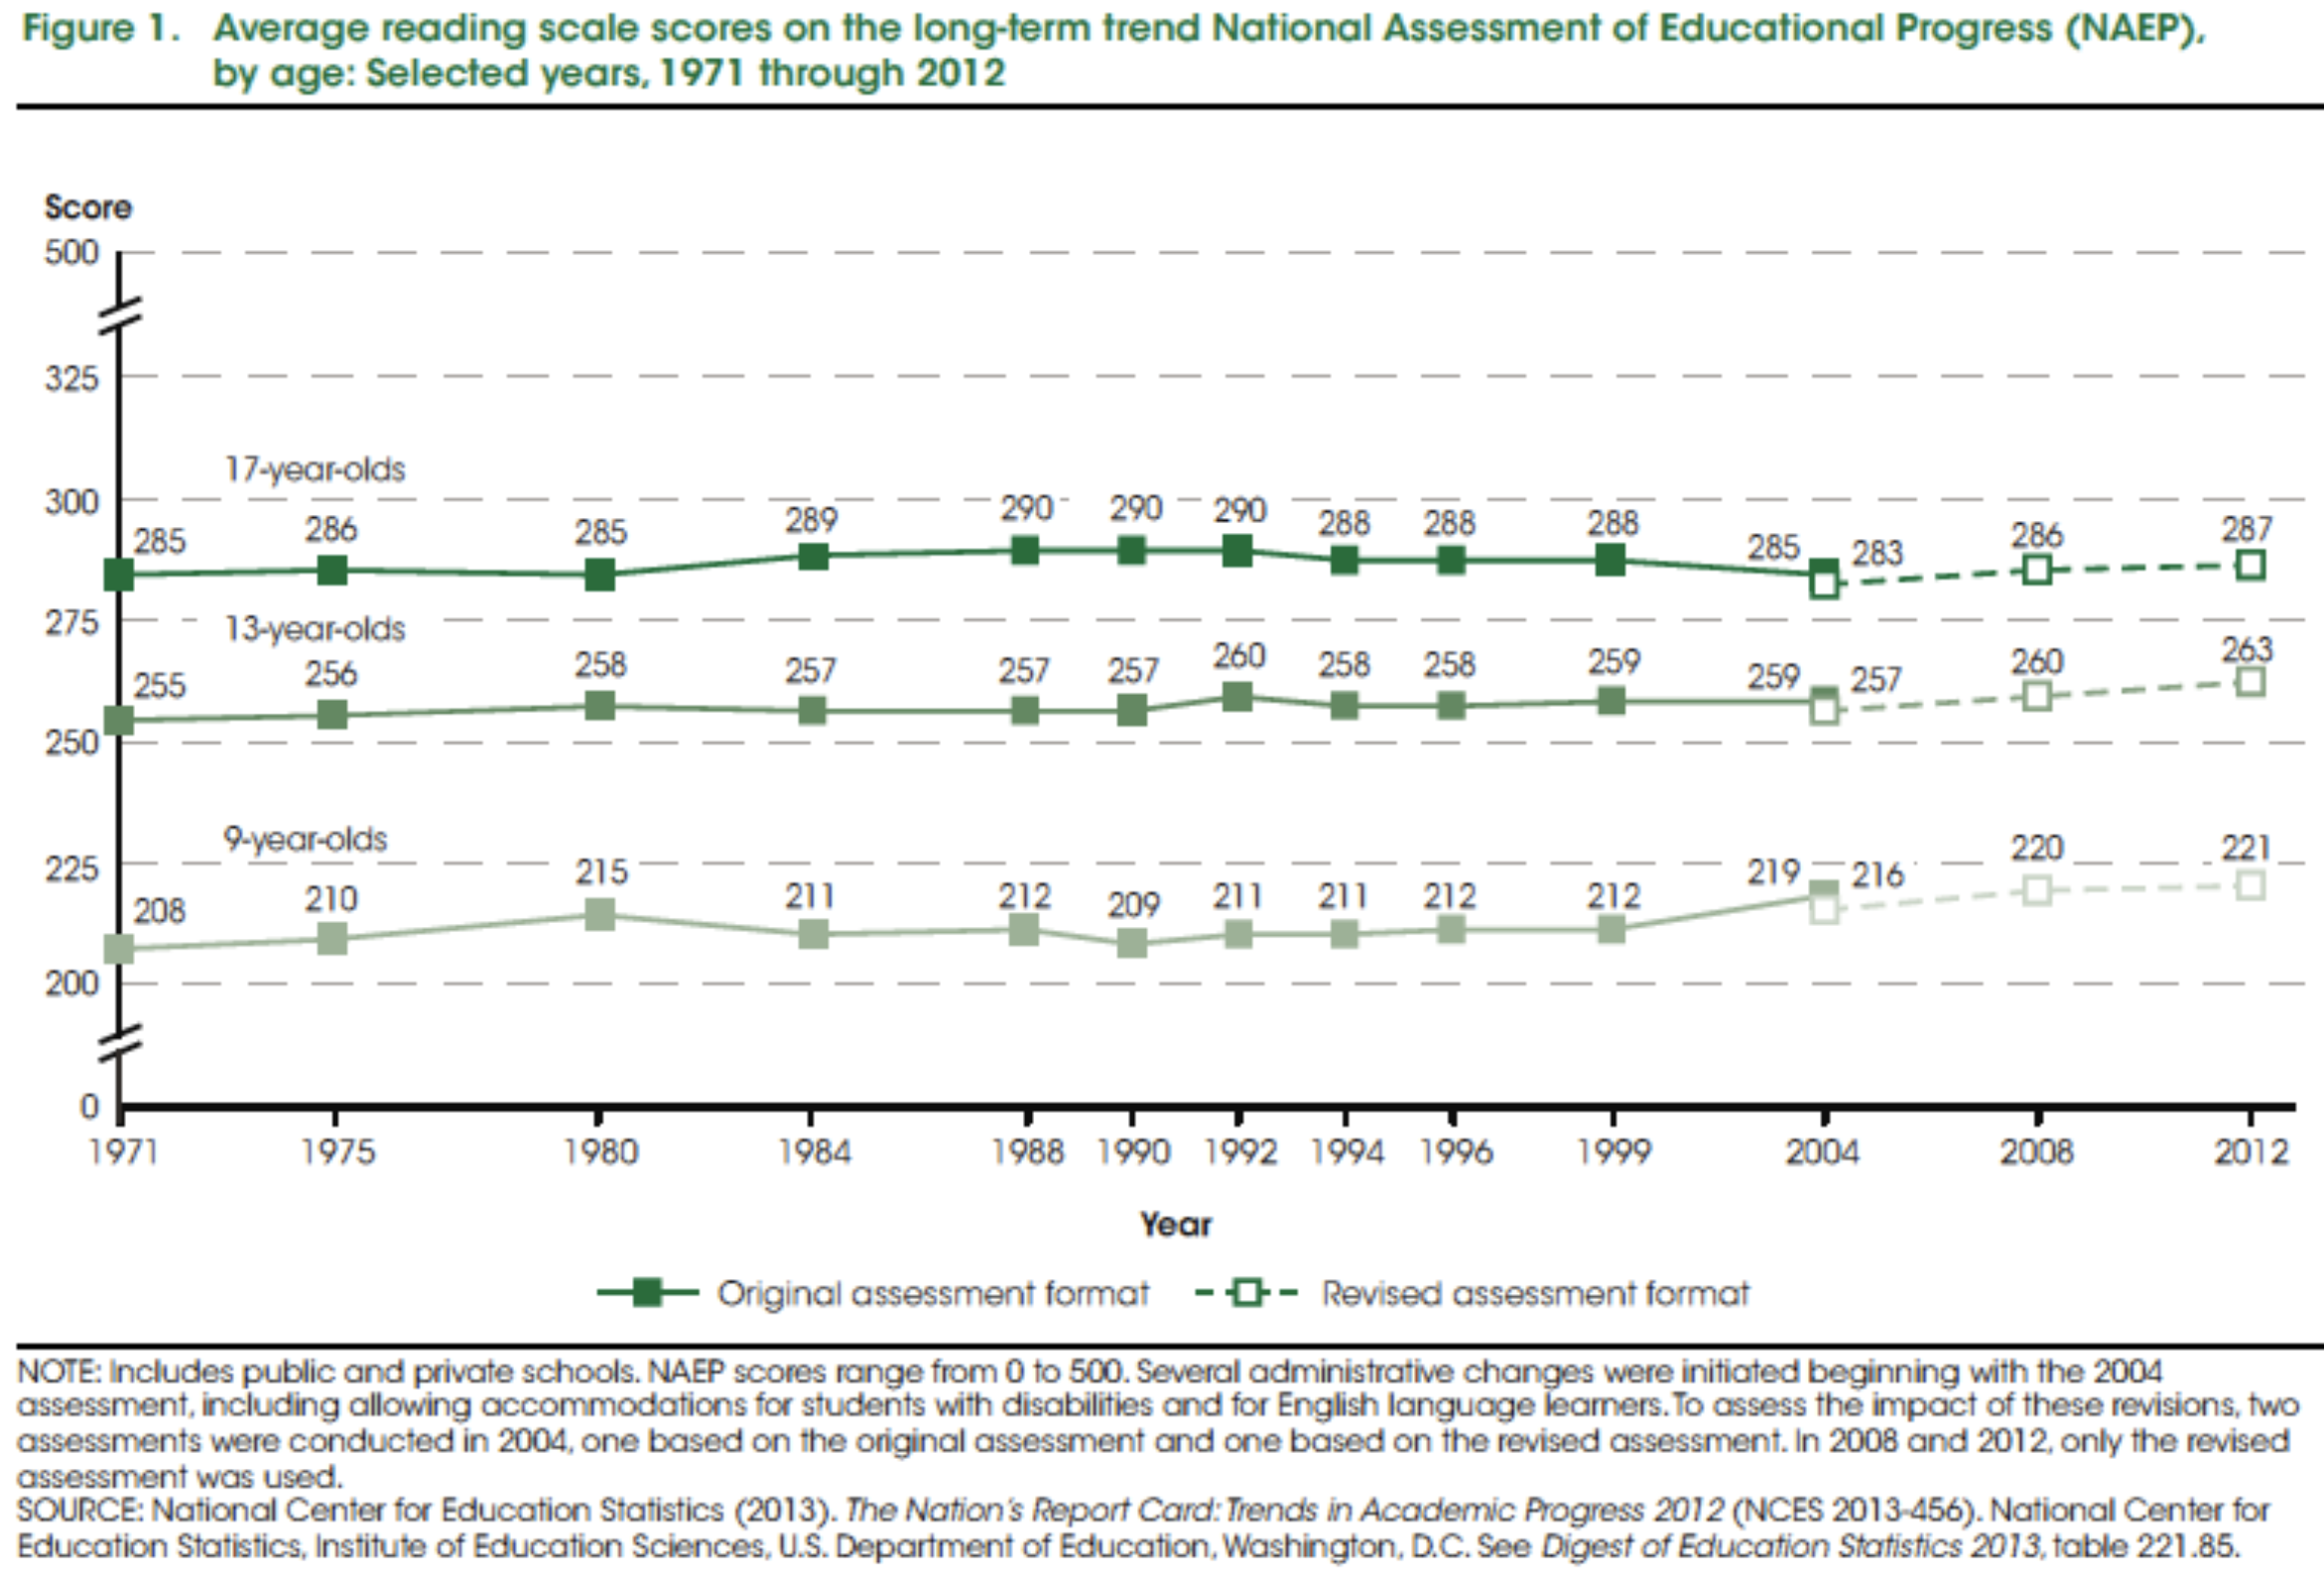
\includegraphics[width=4in]{images/ch9/9 us result 1.png}
                \caption{Average Reading Scale Scores on NAEP by age 1973-2012}
            \end{figure}
            \begin{figure}[H]
                \centering
                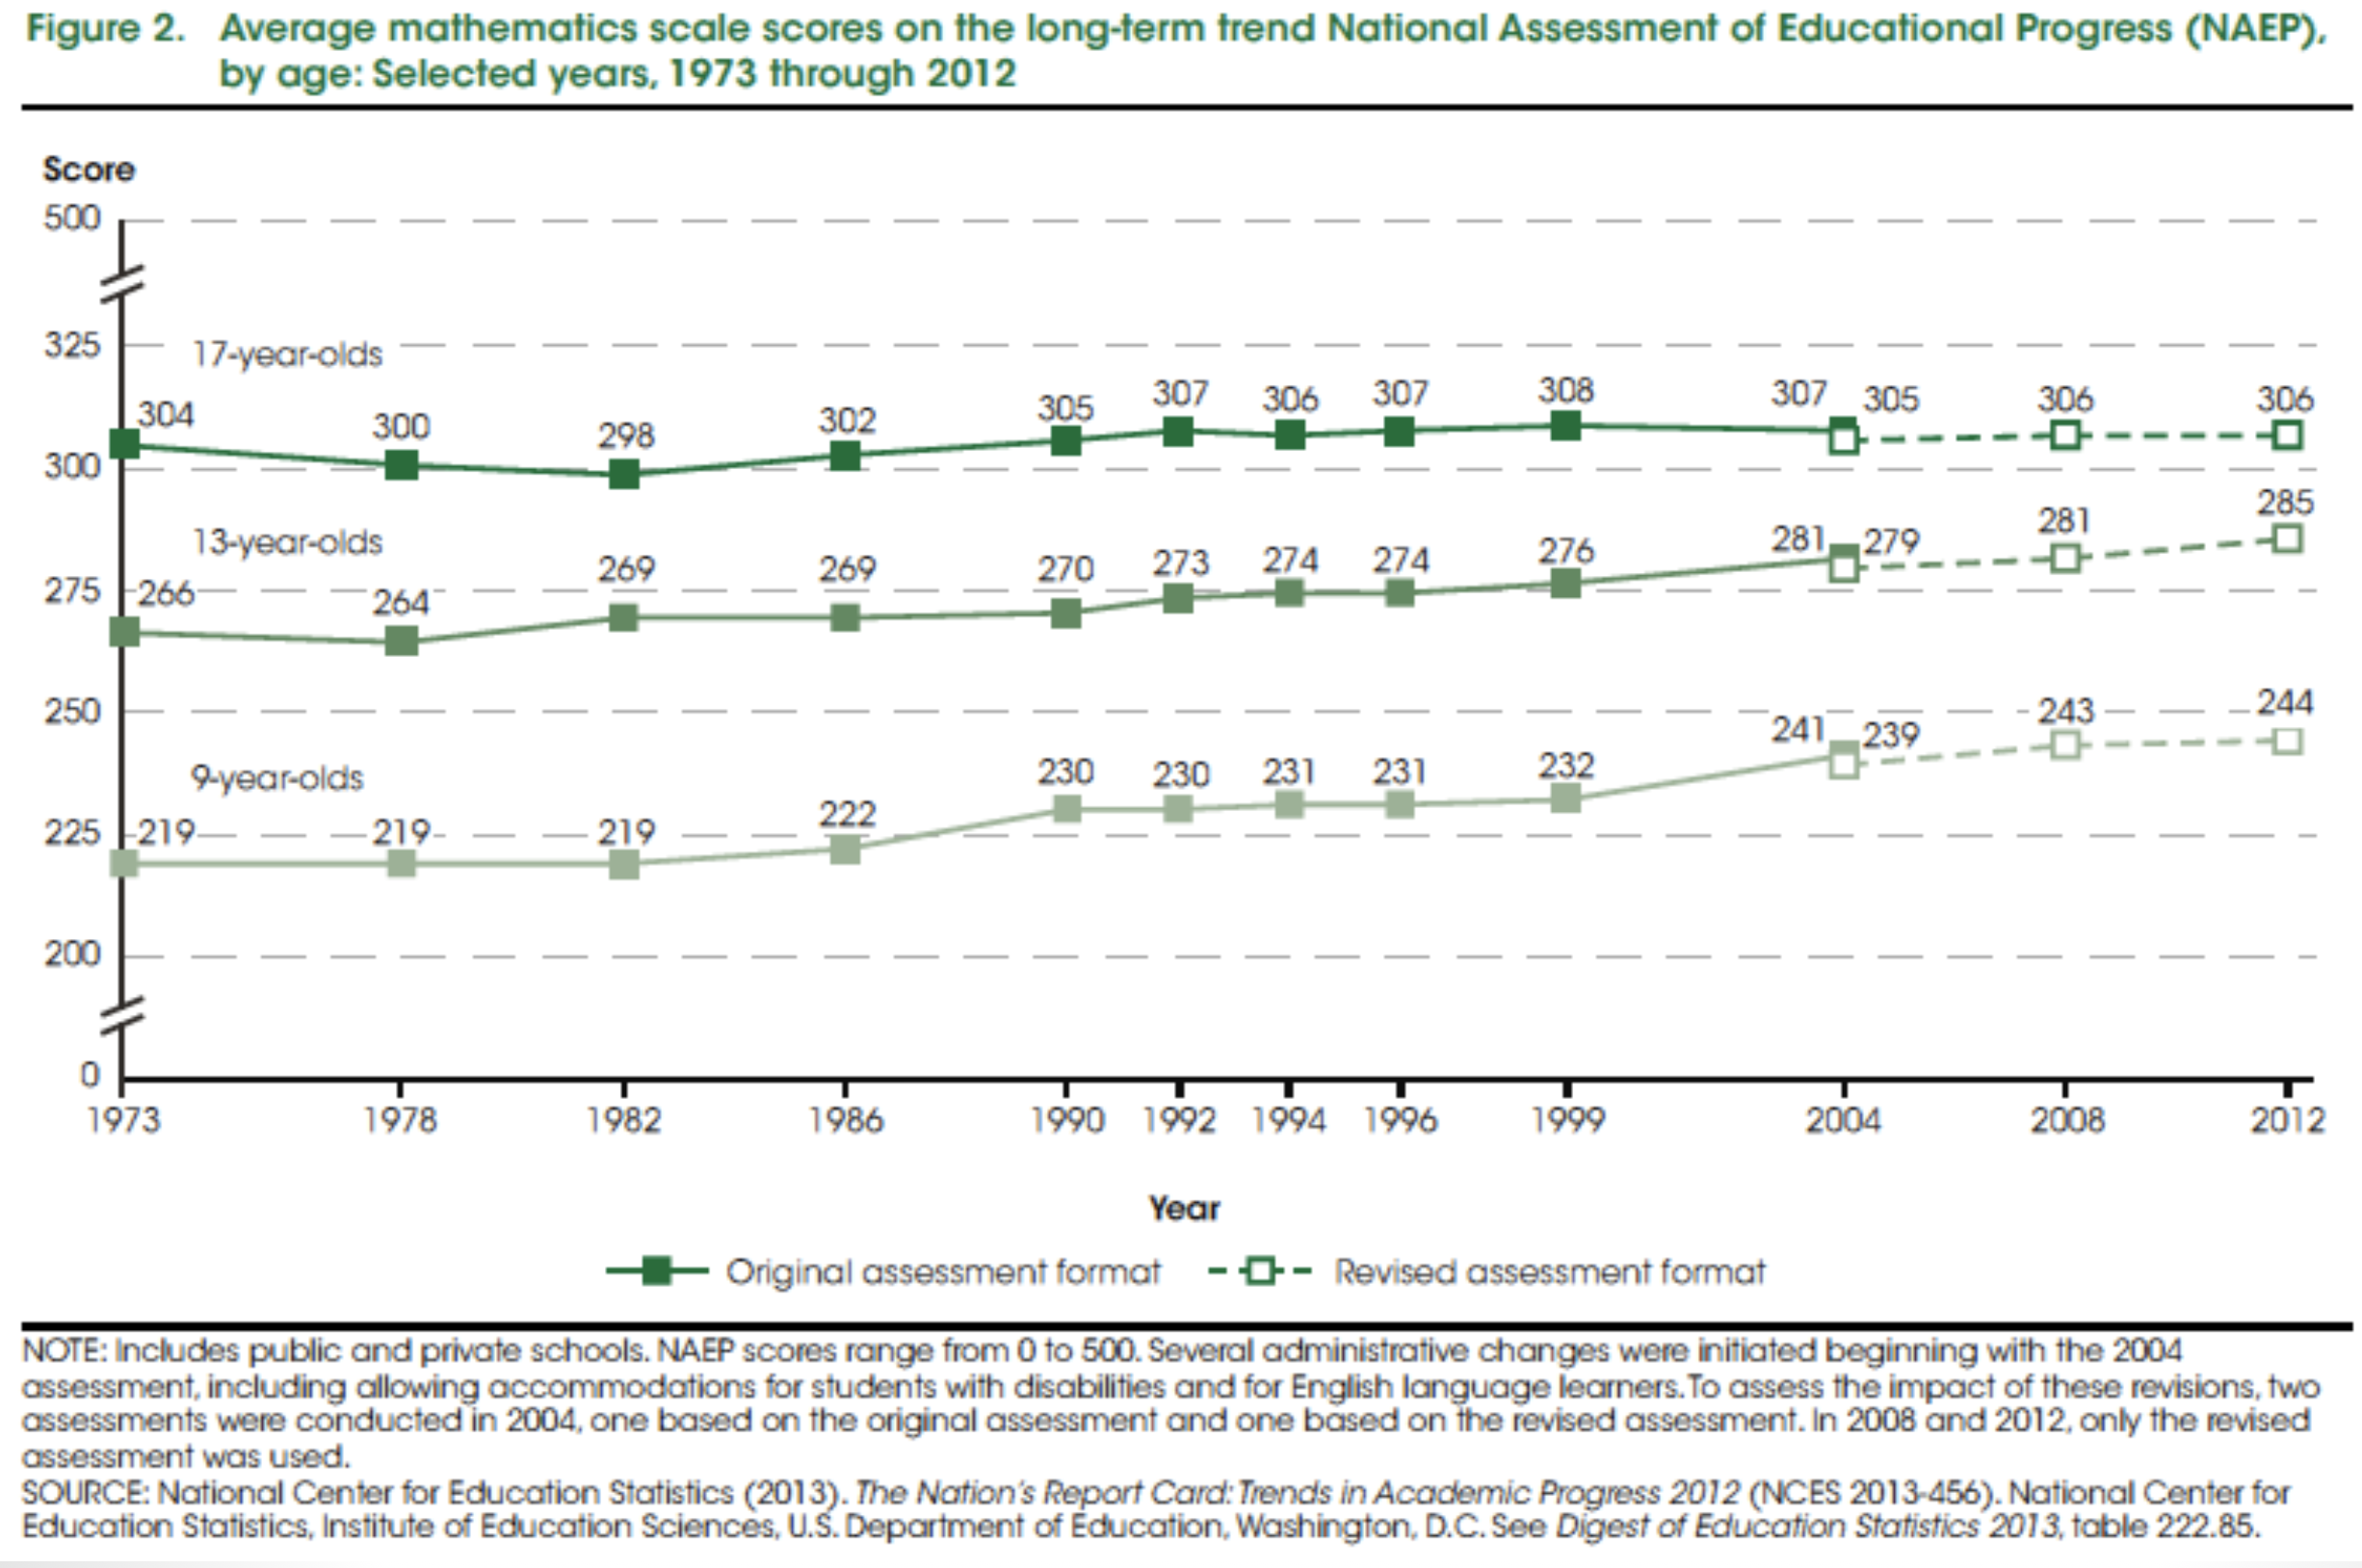
\includegraphics[width=4in]{images/ch9/9 us result 2.png}
                \caption{Average Mathematics Scale Scores on NAEP by age 1973-2012}
            \end{figure}
            However, these was no obvious improvement in education outcomes in U.S.
        
        \subsubsection{School Results in the UK}
            \begin{figure}[H]
                \centering
                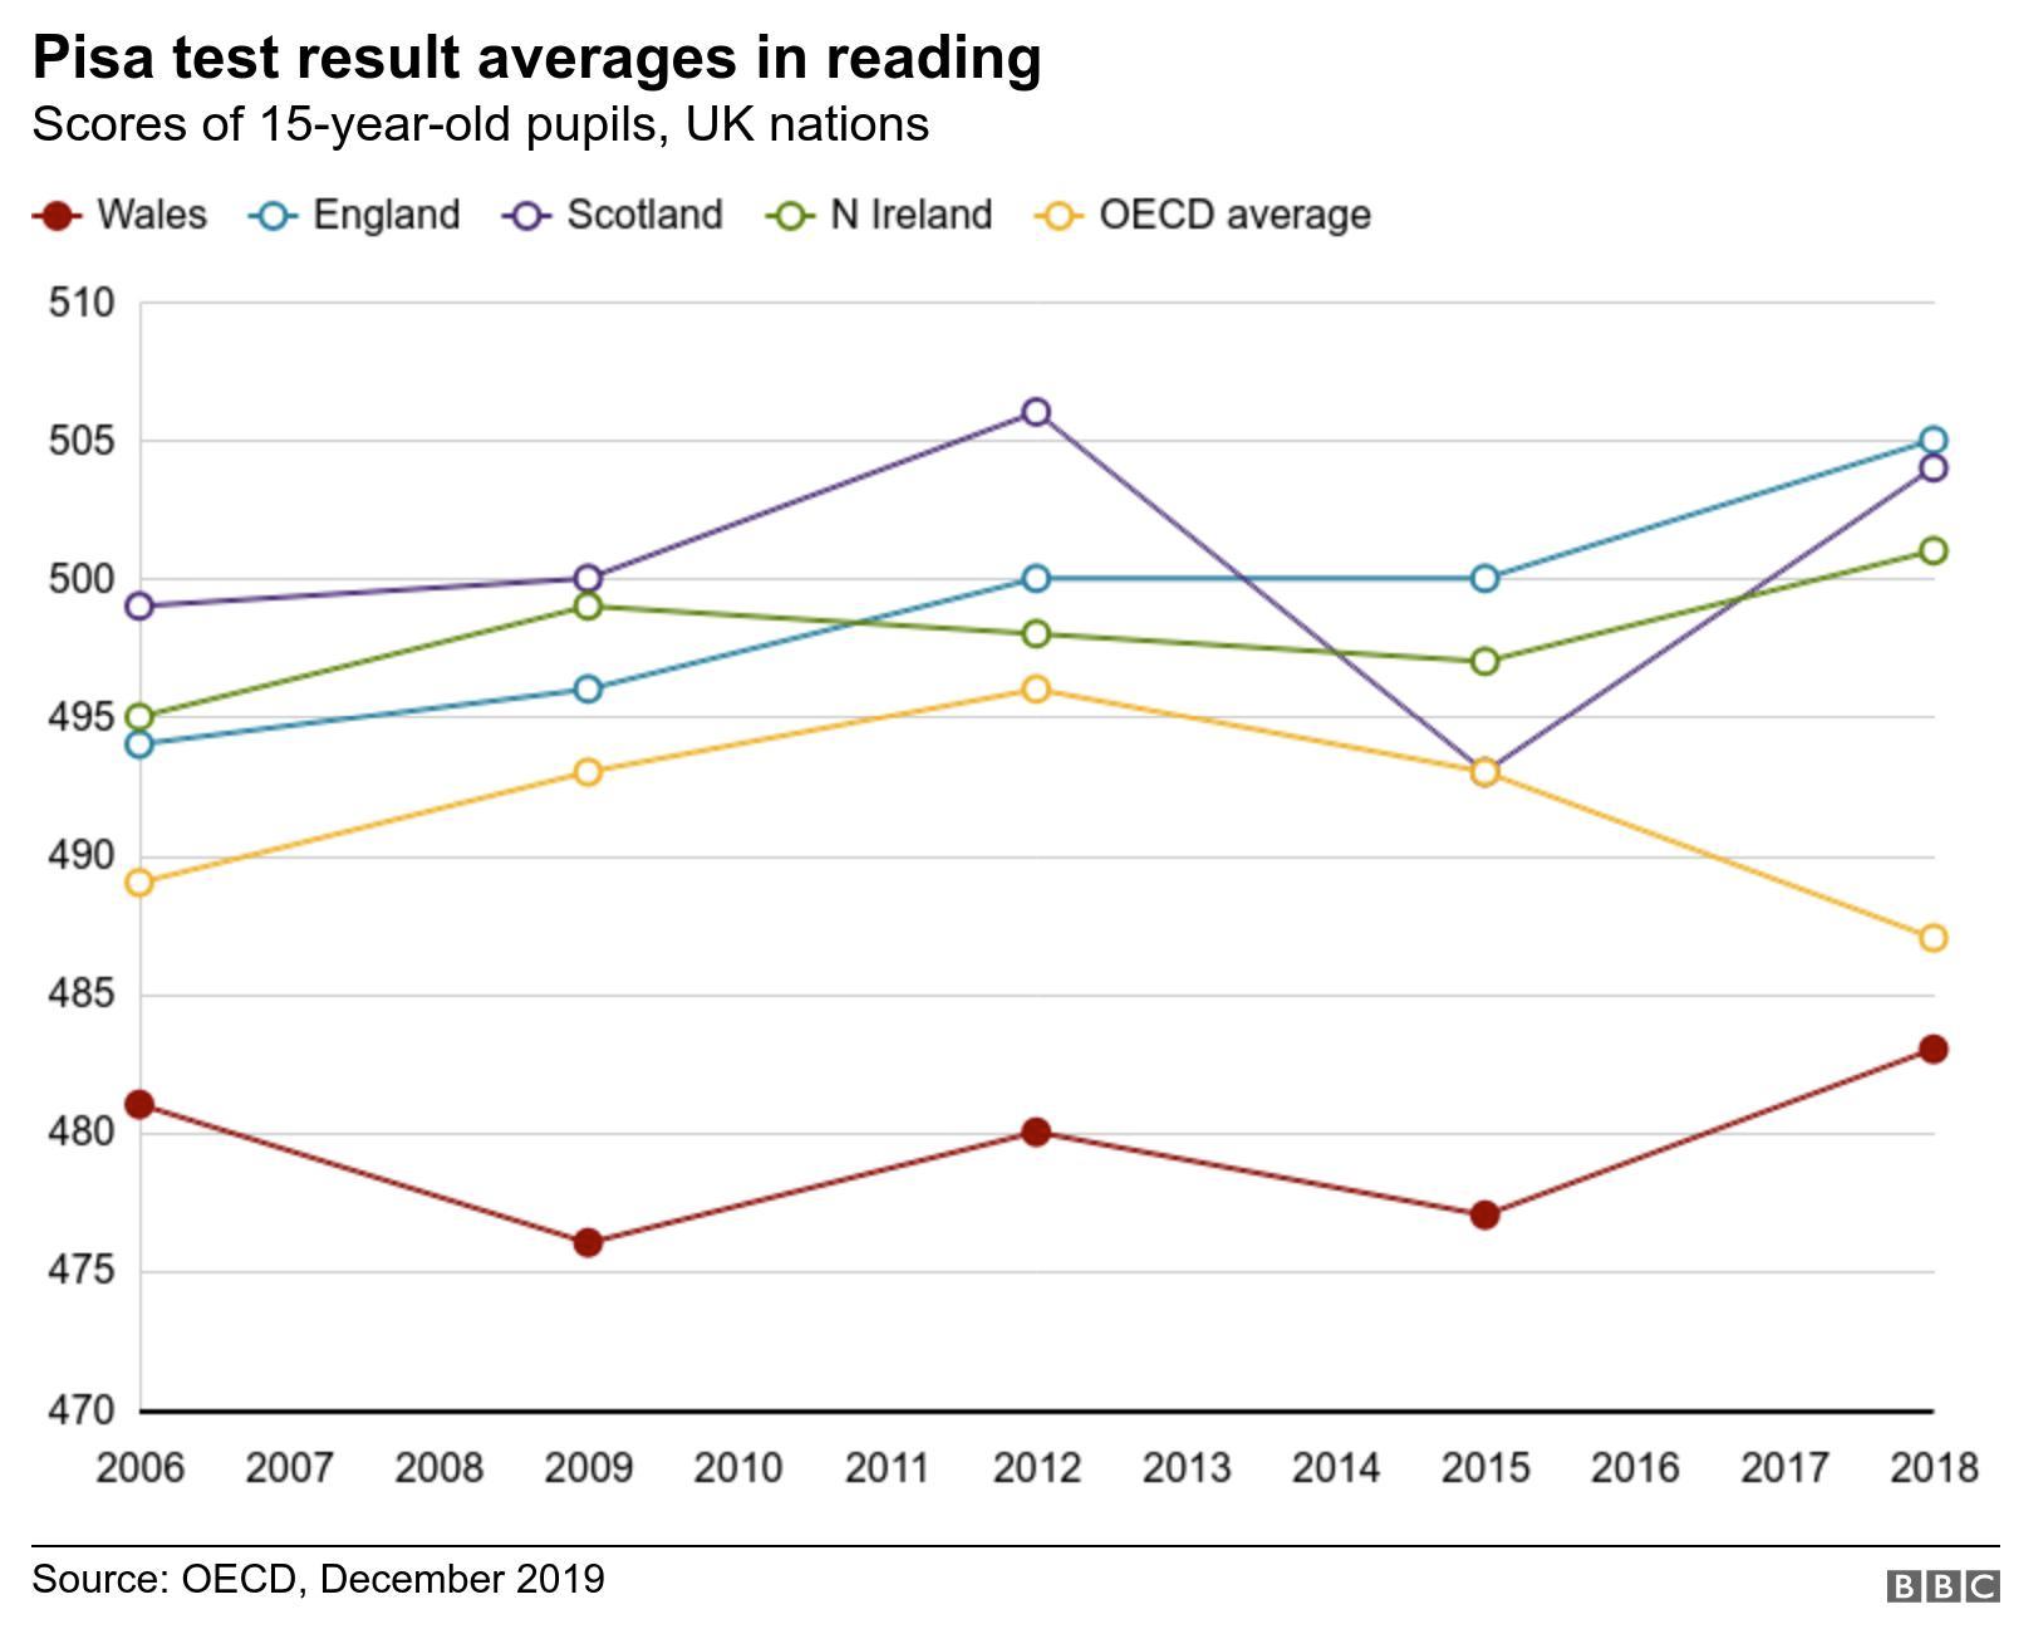
\includegraphics[width=4in]{images/ch9/9 uk result 1.png}
                \caption{PISA Test Result Averages in Reading}
            \end{figure}
            \begin{figure}[H]
                \centering
                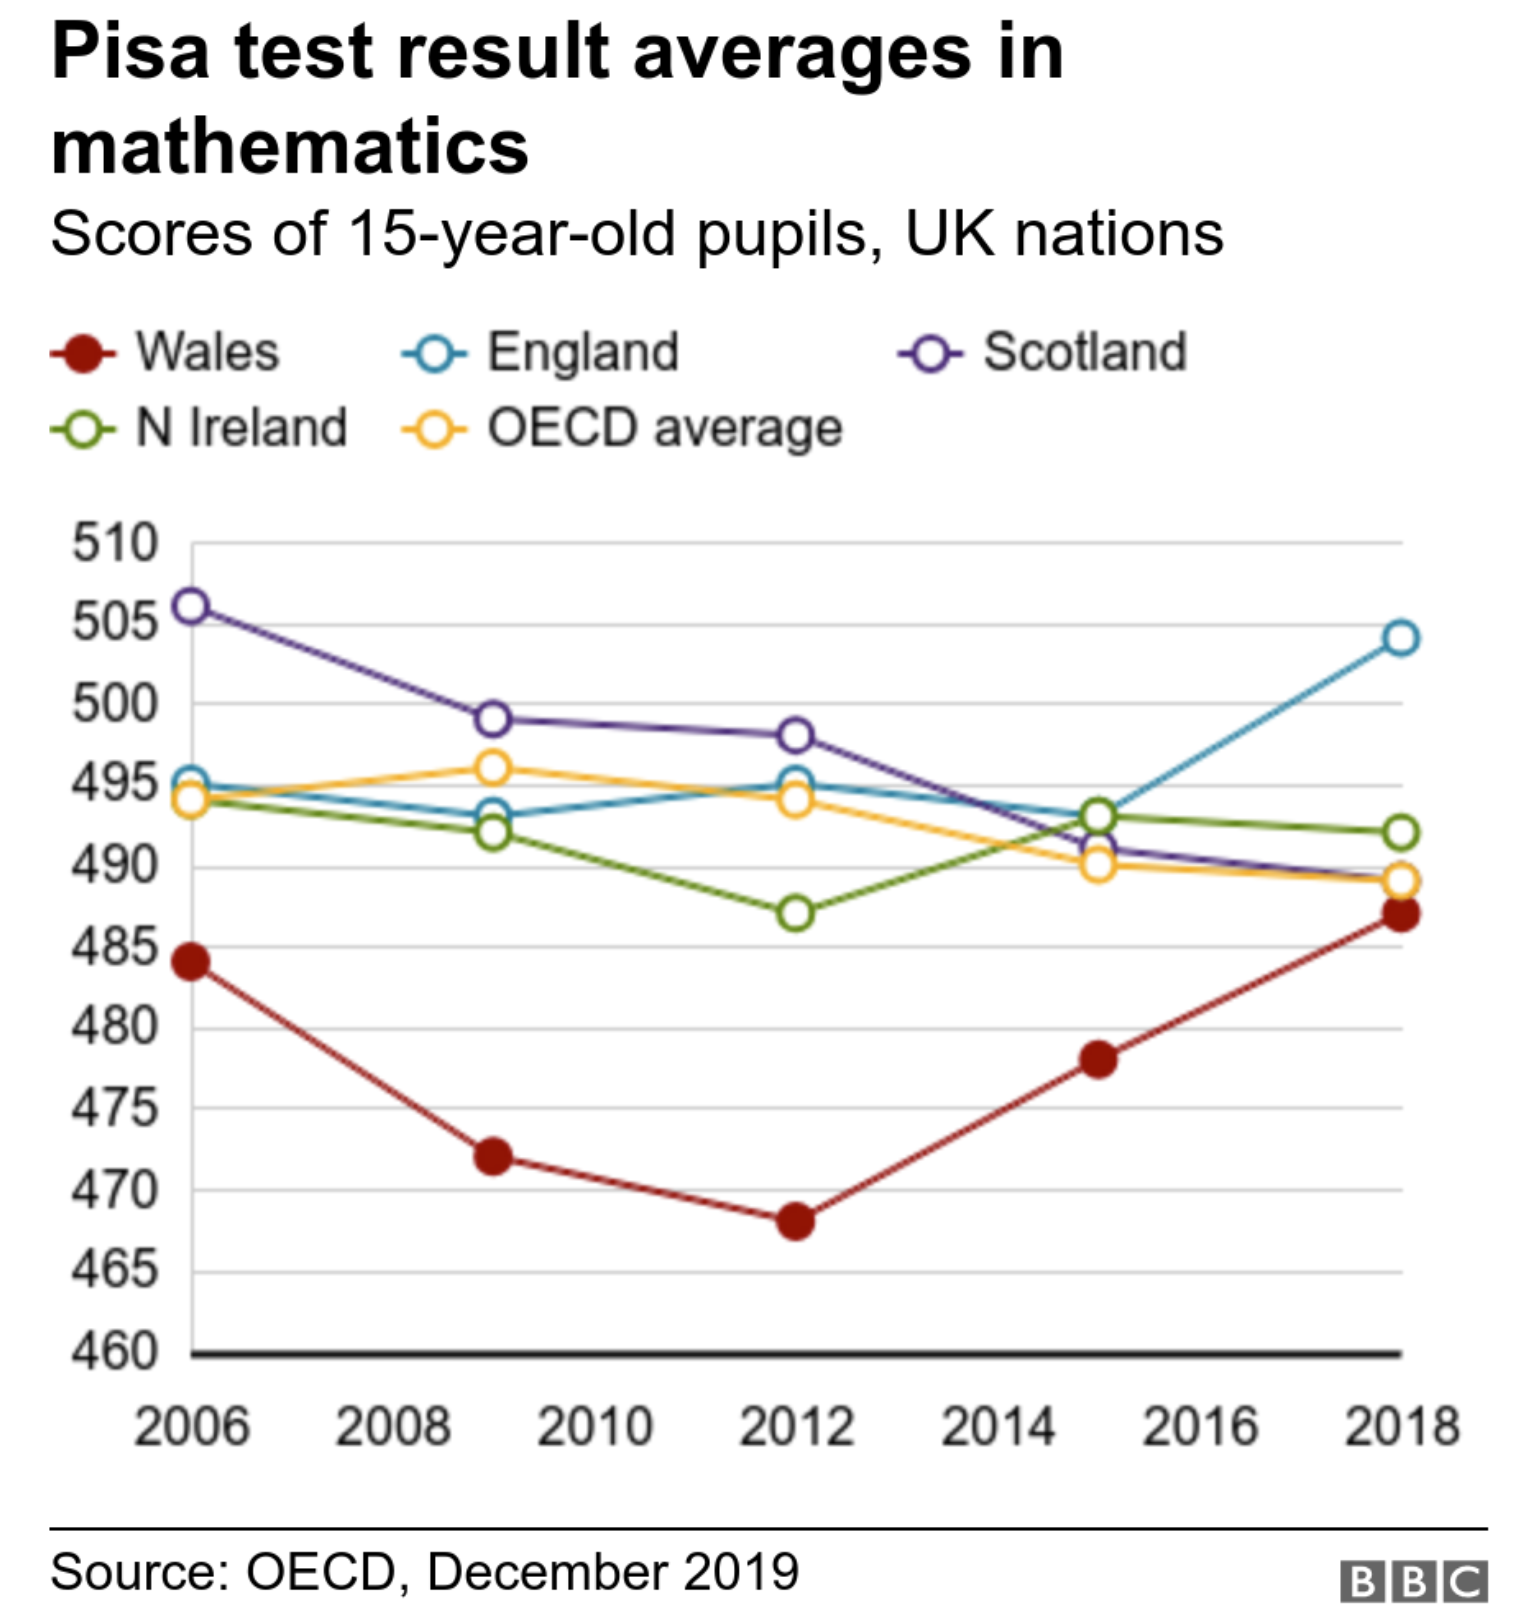
\includegraphics[height=2.5in]{images/ch9/9 uk result 2.png}
                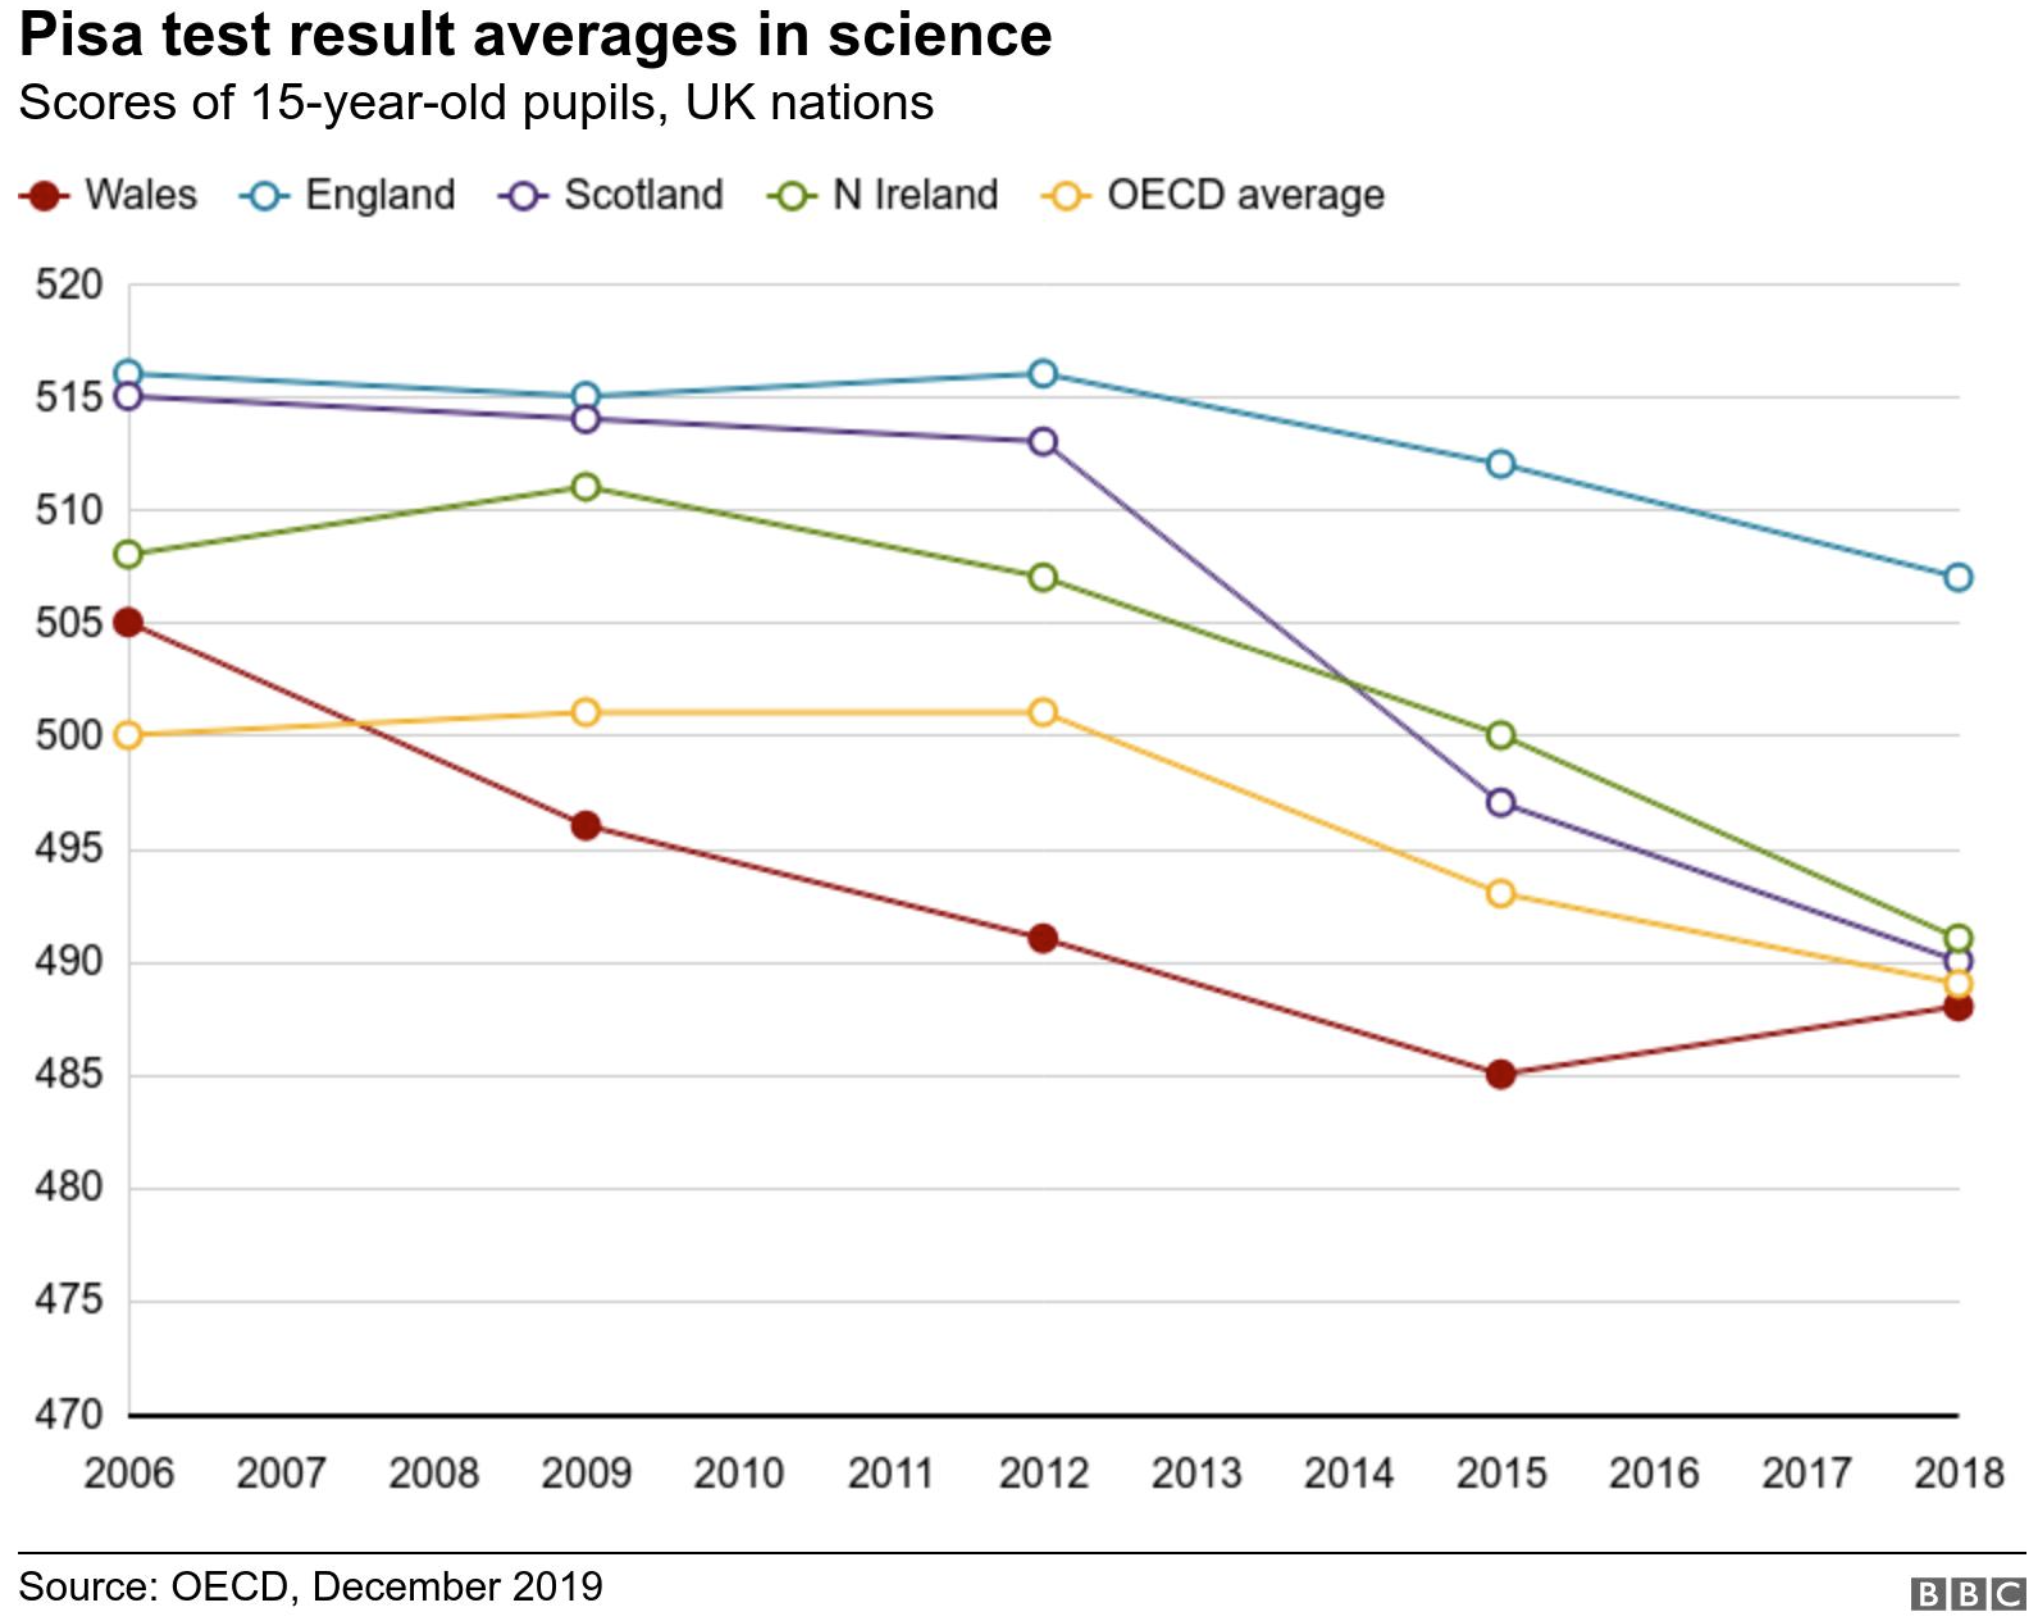
\includegraphics[height=2.7in]{images/ch9/9 uk result 3.png}
                \caption{PISA Test Result Averages in Math and Science}
            \end{figure}
            Similarly, the education outcome in the UK is also stagnant.

\section{$\star$ Measuring Teacher Quality: Standard Value-Added Model}
    
    \subsection{Motivation}
        As seen in the previous section, standard measures of school resources do not seem to predict learning, at least when we look at trends. When we examine more micro studies on specific aspects of school quality, such as class size we seem to find some but small impacts of resources on learning.
        
        Meanwhile, the most important school input is likely to be the teacher. Thus, in the following sections, we will develop measures of teacher quality and examine whether estimated teacher quality predicts student learning.
        
    \subsection{Standard Value-Added Model}
        
        \subsubsection{Introduction}
            There are observable measures of teacher quality, such as experience, education, IQ, grades, etc., but they do not predict student learning. Thus, at least at a practical level, important teacher attributes seem to be essentially unobserved.
            
            Therefore, we \emphb{define teacher quality as the amount of learning observed in students taught by a particular teacher}.
            
            The basic idea is to measure the performance of students in two tests across a time interval, take average of all students of a given teacher, and call that teacher quality. This is similar to the \emphb{league tables} in the UK.

            \empha{Since this measure does not have an exact scale, we calculate the variance / standard deviation and use that as a scale.}
            
        \subsubsection{Setup}
            \begin{equation}
                \color{red}
                A_{ijt} = \theta A_{ij,t-1} + \gamma X_{ijt} + \alpha_{jt} + \epsilon_{ijt}
                \tag{Standard Value-Added Model}
                \label{eqn:edu_value_add_m}
            \end{equation}
            where:
            \begin{itemize}
                \item $i$: student; $j$: teacher; $t$: grade
                \item $\theta$: scaling factor (to make tests comparable)
                \item $A_{ijt}$: student achievement
                \item $X_{ijt}$: student characteristics
                \item \empha{$\alpha_{jt}$: teacher $j$'s fixed effect in period $t$ (teacher quality)}
            \end{itemize}
            $\alpha$ measures the teacher quality: it is the average learning of students of teacher $j$.
            
            This could be written in another way:
            \begin{equation*}
                \underbrace{A_{ijt} - \theta A_{ij,t-1}}_{\text{Value Added}} = \gamma X_{ijt} + \alpha_{jt} + \epsilon_{ijt}
            \end{equation*}
        
    \subsection{Interpretation and Scale}
        
        \subsubsection{Interpretation and Distinguish Classroom FE}
            $\alpha$ is really a fixed effect of a regression -- it measures the average performance of students taught by a particular teacher, and we call it teacher quality.
            
            Therefore, we will need to observe at least 2 groups of students taught by the same teacher in order to distinguish classroom/peer fixed effects and teacher fixed effects. \empha{If only observe one group per teacher, $\alpha$ combines both classroom/peer and teacher FE.}
        
        \subsubsection{Scale}
            The magnitude of $\alpha$ does not have a direct interpretation. Thus, we compute the standard deviation of $\alpha$, noted as $\sigma_\alpha$, and use it as the unit for $\alpha$.

            For instance, $\alpha=1$ means that an 1 $\sigma_\alpha$ increase in teacher quality will induce an 1 $\sigma_A$ increase in students' value added. Put it differently, $\alpha$ is the change in student achievement measured in $\sigma_A$ corresponding to an 1 $\sigma_\alpha$ increase in the teacher quality.
        
    
    \subsection{Example}

        \begin{figure}[H]
            \centering
            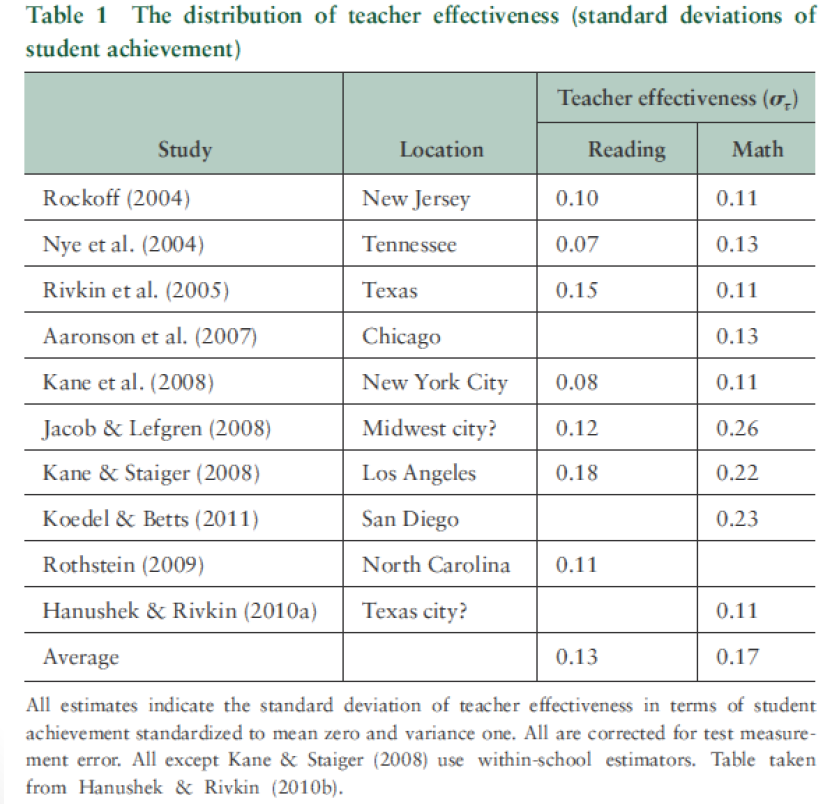
\includegraphics[width=4in]{images/ch9/9 hanushek rivkin.png}
            \caption{Distribution of Teacher Effectiveness}
        \end{figure}
        

\section{$\star$ Non-Random Sorting / Selection}
    
    \subsection{Student Sorting / Selection}
        Our standard value-added model introduced above depends on the critical assumption of \emphb{conditional random assignment}: conditional on $A$ and $X$, the assignment of students to teachers is random:
        $$(A_{0,ijt},A_{1,ijt})\perp \mathds{1}[j=J]|A_{ij,t-1},X_{ijt}$$
        This requires us to include all characteristics that jointly affect selection and outcome. In other words, we cannot have selection on unobservables.
        
    \subsection{Rothstein 2010: Evidence on Non-random Sorting}
        \cite{rothstein_teacher_2010} questioned the conditional random assignment assumption. He checked whether future teacher assignments predict current student learning, which is similar to a placebo test.

        The intuition is simple: if the 5th grade teacher predicts 4th grade learning, this could only be caused by non-random sorting of students to teachers, because teachers cannot influence students retrospectively.

        Specifically, instead of estimating the \ref{eqn:edu_value_add_m}, he estimates the following model:
        \begin{equation*}
            \color{red}
                A_{ikt-1} = \theta A_{ik,t-2} + \gamma X_{ikt-1} + \alpha_{jt} + \epsilon_{ikt-1}
        \end{equation*}

        He rejects that $\alpha_{jt}$'s are jointly equal to zero, and the standard error of $\alpha_{jt}$ is about 0.08 instead of around 0.1 estimated with standard models. This suggests that there is \emphb{non-random sorting}.
        
    \subsection{Chetty, Friedman, Rockoff 2014: Bias is Small}

        \subsubsection{Setup}
            \cite{chetty_measuring_2014-1} confirms that \cite{rothstein_teacher_2010} is correct, but the \emphb{resulting bias is small}.
    
            Chetty et al. look at quasi-experiments -- changes in teachers across schools.
    
            Specifically:
            \begin{itemize}
                \item 2 schools: school $A$ and school $B$
                \item 2 teachers: teacher $a$ works in school $A$, and teacher $b$ works in school $B$
                \item $\alpha_{aA}$ is the estimated value added for teacher $a$ in school $A$
                \item $\alpha_{bB}$ is the estimated value added for teacher $b$ in school $B$
                \item Teacher $a$ moves to school $B$
            \end{itemize}
            Then, after the movement of teacher $a$, the change in students' learning should be the same as the change in mean teacher value-added ($\alpha _{a}-\alpha_{b}$), assuming teacher movements are random. Otherwise, there is likely to be bias in value added estimates due to sorting.

        \subsubsection{Results}
            \begin{figure}[H]
                \centering
                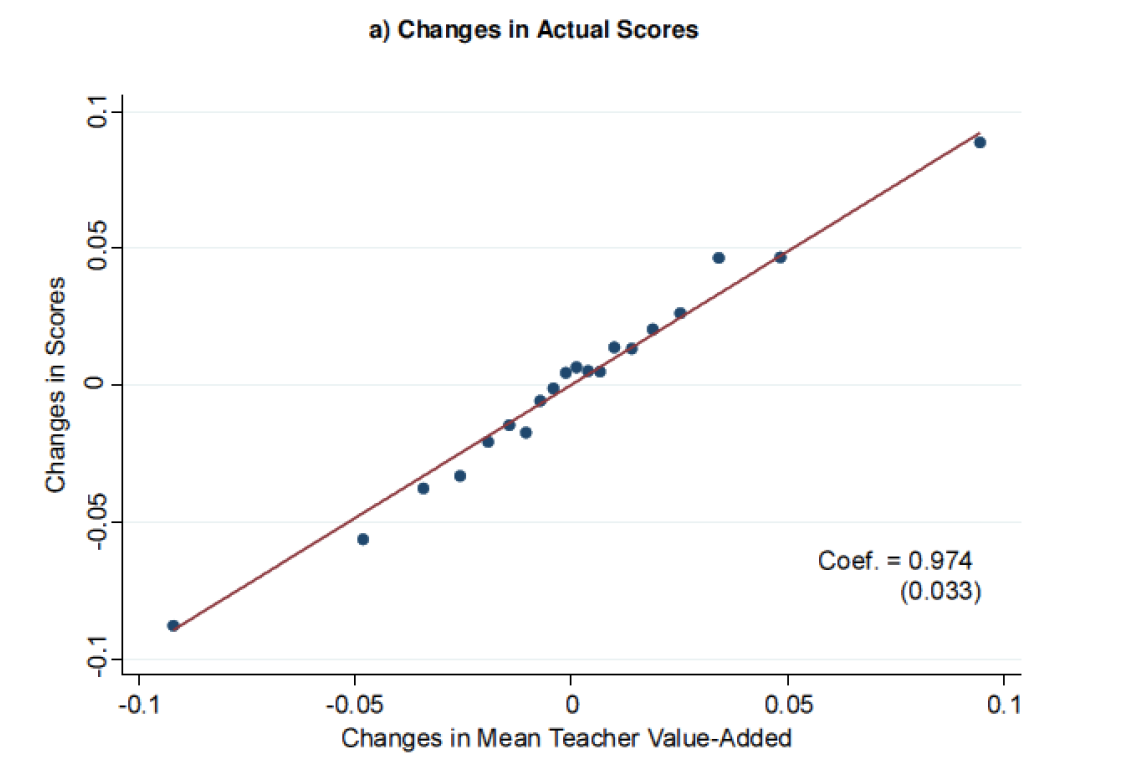
\includegraphics[width=4in]{images/ch9/9 chetty 2014.png}
                \caption{Change in Actual Scores and Changes in Mean Teacher Value-Added (\cite{chetty_measuring_2014})}
            \end{figure}
            The movement is nearly one-to-one, so bias due to non-random sorting is very small.

        \subsubsection{But Still Not Settled}
            There are follow-up discussions from Rothstein and Chetty, Friedman and Rockoff regarding whether changes in teachers is correlated with prior achievement gains of students (or can we say that they are essentially random)?
    
    \subsection{Kane et al. 2013: Additional Evidence from Random Assignment}

        \cite{kane_have_2013} randomly assigned students to teachers in 2011, ensuring there is no systematic sorting of students to teachers. Then, they check how will estimate of value-added in 2009-10 predicts student learning in 2011. The result show that the prediction is well good, which indicates there's \empha{no sorting}.

        \begin{figure}[H]
            \centering
            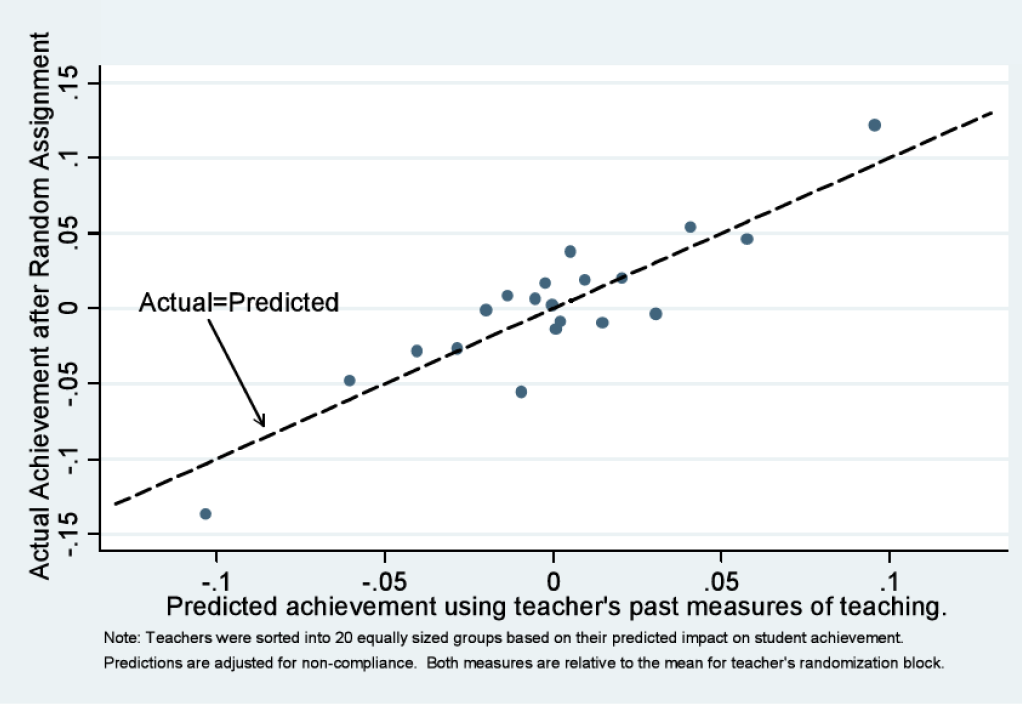
\includegraphics[width=4in]{images/ch9/9 kane math.png}
            \caption{Actual and Predicted Achievement in Maths (\cite{kane_have_2013})}
        \end{figure}
        \begin{figure}[H]
            \centering
            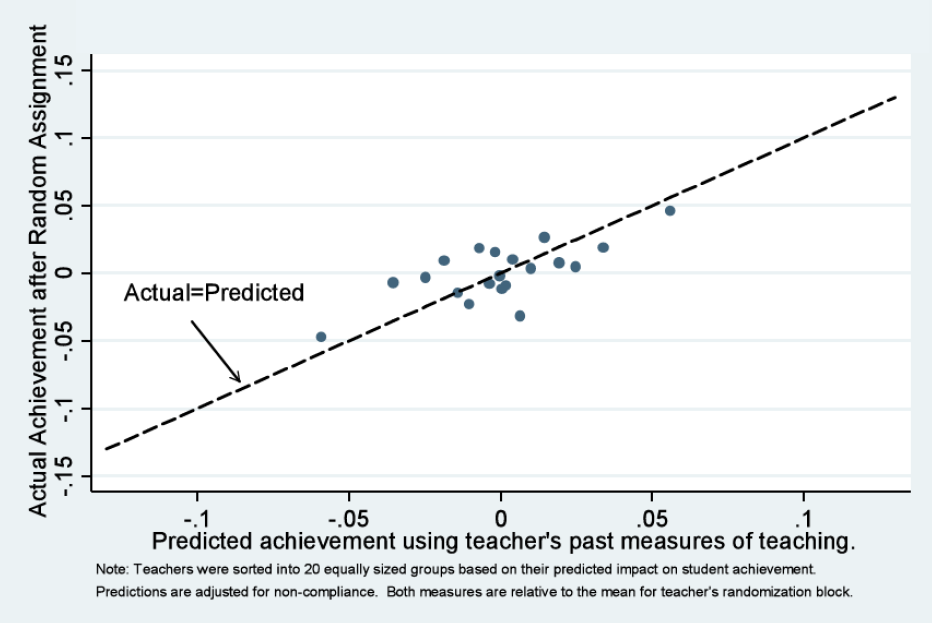
\includegraphics[width=4in]{images/ch9/9 kane arts.png}
            \caption{Actual and Predicted Achievement in Arts (\cite{kane_have_2013})}
        \end{figure}
        
\section{$\star$ Measurement Issues}

    \subsection{Measurement Error}

        In the \ref{eqn:edu_value_add_m}, suppose $\alpha_{jt}=\alpha_{j}$ (time-unvarying), we cannot observe $\alpha_j$ directly. Instead, we need to estimate it. This comes with a \emphb{measurement error} $v_j$ due to sampling uncertainty (with data from more years, this could be smaller):
        $$\widehat{\alpha_j}=\alpha_j + v_j$$
        Therefore, assume the measurement error $v_j$ is independent of $\alpha_j$:
        $$Var(\widehat{\alpha_j})=Var(\alpha_j)+Var(v_j)$$
        
        Hence, $Var(\widehat{\alpha_j})$ overestimates $Var(\alpha_j)$. If the variance of measurement error is large, it will be hard/unreliable to rank teachers based on $\widehat{\alpha_j}$.

    \subsection{Dealing with Measurement Error: Empirical Based Error Correction}

        We can use the law of total variance to get an estimate of $Var(v_{j})$ and use it to retrieve $Var(\alpha_j)$:
        $$Var(\widehat{\alpha_j})=\underbrace{Var(E[\widehat{\alpha_j}|j])}_{\approx Var(\alpha_j)}+\underbrace{ E[Var(\widehat{\alpha_j}|j)] }_{ \approx Var(v_{j}) }$$
        $$Var(\alpha_j)\approx Var(\widehat{\alpha_j})-E[Var(\widehat{\alpha_j})|j]$$
        Here, $E[Var(\widehat{\alpha_j})|j]$ is just the variance of the FE, which could be obtained from the regression. Using it to proxy $Var(v_j)$, we can retrieve $Var(\alpha_j)$.
        
        However, this method cannot filter out variance from classroom FE shocks. With richer data, we may consider the next method.
        
    \subsection{Dealing with Measurement Error and Distinguish Teacher / Classroom Effects}

        If we have \empha{data of multiple years}, this alternative method can deal with measurement error while distinguish teacher and classroom effects at the same time.

        Firstly, we estimate the \ref{eqn:edu_value_add_m} for multiple years ($t \neq s$) and get:
        \begin{itemize}
            \item $\widehat{\alpha_{jt}}=\alpha_j + w_{jt} + v_{jt}$
            \item $\widehat{\alpha_{js}}=\alpha_j + w_{jt} + v_{js}$
        \end{itemize}
        where:
        \begin{itemize}
            \item $\alpha$ is teacher's value added (teacher effect)
            \item $w$ is classroom effect
            \item $v$ is sampling error
        \end{itemize}
        Assume that:
        \begin{itemize}
            \item Classroom shocks are serially uncorrelated and independent of $\alpha_j$: $Cov(w_{jt},w_{js})=0, (w_{jt},w_{js})\perp \alpha_j$
            \item Sampling errors are serially uncorrelated and independent of $\alpha_j$: $Cov(v_{jt},v_{js})=0, (v_{jt},v_{js})\perp \alpha_j$
        \end{itemize}
        Then, we can calculate $Var(\alpha_j)$ by:
        $$Cov(\widehat{\alpha_{jt}},\widehat{\alpha_{js}}) = Cov(\alpha_j,\alpha_j) + \underbrace{Cov(\alpha_j,w_{jt}+v_{jt}) + Cov(\alpha_j,w_{js}+v_{js}) +Cov(w_{jt}+v_{jt},w_{js}+v_{js})}_{0} = Var(\alpha_j)$$

        The previous method can only eliminate $Var(v_{jt})$ and retrieve $Var(\alpha_j + w_{jt})$, which is a mixture of teacher/classroom FE, but this alternative method can also eliminate the variance of classroom FE.
        
    \subsection{Fluctuations in Teacher Quality}

        \cite{chetty_measuring_2014} extended the model to allow for $\alpha_j$ to vary over time. Specifically, they use $\{ \alpha_{jt-T},\dots,\alpha_{jt-1} \}$ to predict $\alpha_jt$.

\section{Predictors of Teacher Quality}

    \subsection{Rockoff et al. 2008: Observed Characteristics?}

        \subsubsection{Summary}

            Question: can you recognise an effective teacher whe you recruit one?
    
            \cite{rockoff_can_2011} collect several teacher characteristics and correlate the, with $\alpha_j$. The characteristics they collect include:
            \begin{itemize}
                \item Traditional: education, training, college major, SAT scores, ranking of college attended
                \item Non-Traditional: cognitive ability, math knowledge, personal traits, Haberman pre-screener
            \end{itemize}
            The outcome variables are: student test scores in math, teacher absences, subjective evaluations of teachers, whether teacher returns to DOE in the following year, whether  teacher returns to school in the following year.
    
            Results: \empha{most characteristics are not significantly correlated with outcomes at all. Even for those with significant correlations, the magnitudes are tiny.}

        \subsubsection{Specific Results}

            \begin{figure}[H]
                \centering
                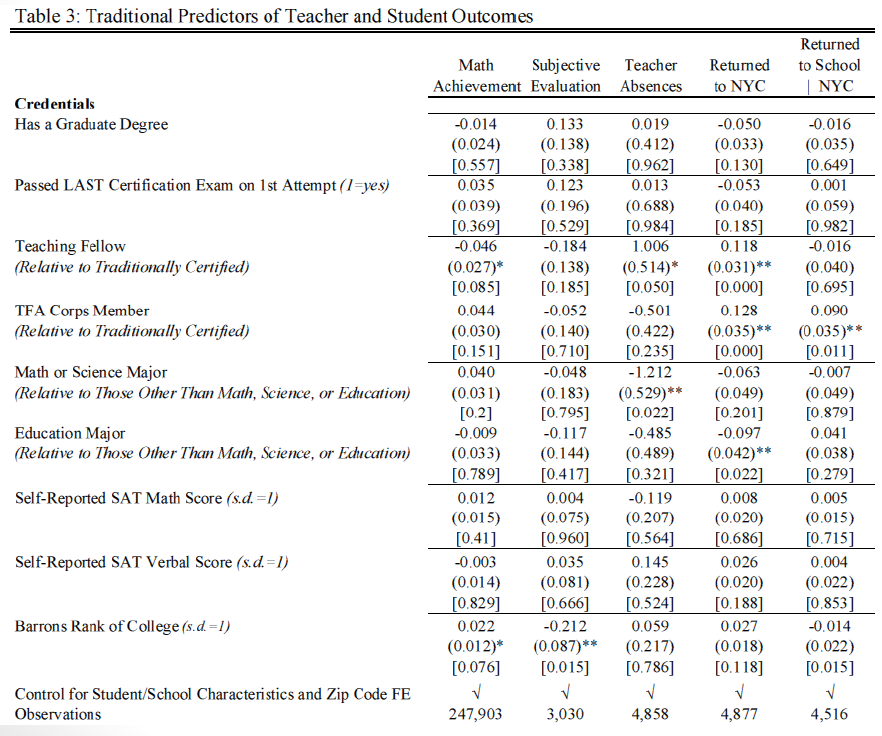
\includegraphics[width=4in]{images/ch9/9 rockoff 1.png}
                \caption{Traditional Predictors of Teacher and Student Outcomes}
            \end{figure}
            \begin{figure}[H]
                \centering
                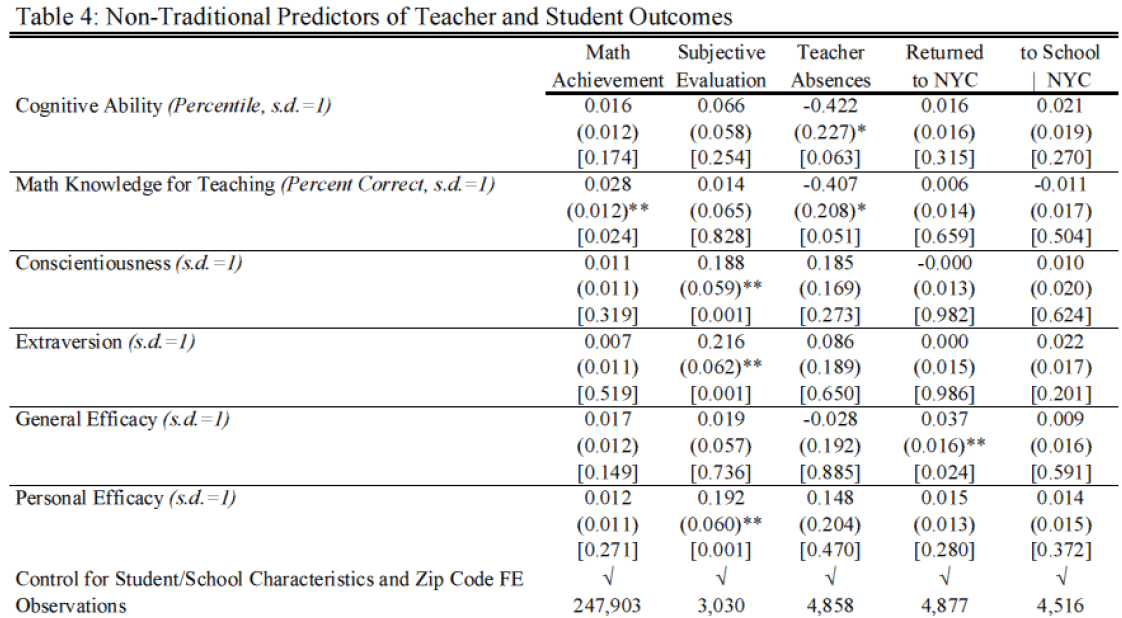
\includegraphics[width=4in]{images/ch9/9 rockoff 2.png}
                \caption{Non-Traditional Predictors of Teacher and Student Outcomes}
            \end{figure}
            \begin{figure}[H]
                \centering
                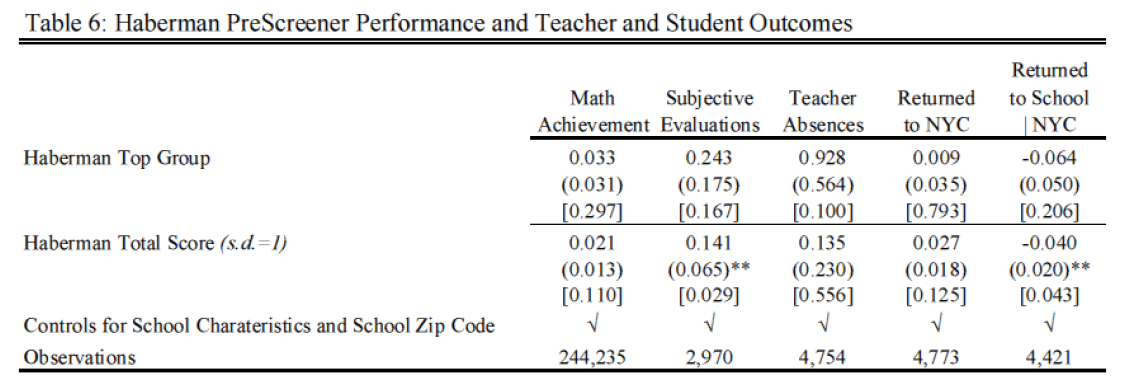
\includegraphics[width=4in]{images/ch9/9 rockoff 3.png}
                \caption{Haberman PreScreener Performance and Teacher and Student Outcomes}
            \end{figure}
            \begin{figure}[H]
                \centering
                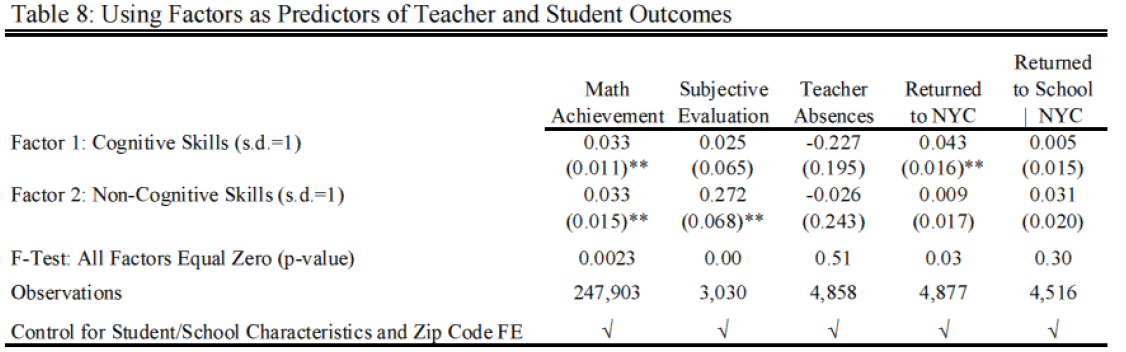
\includegraphics[width=4in]{images/ch9/9 rockoff 4.png}
                \caption{Using Factors as Predictors of Teacher and Student Outcomes}
            \end{figure}
            \begin{figure}[H]
                \centering
                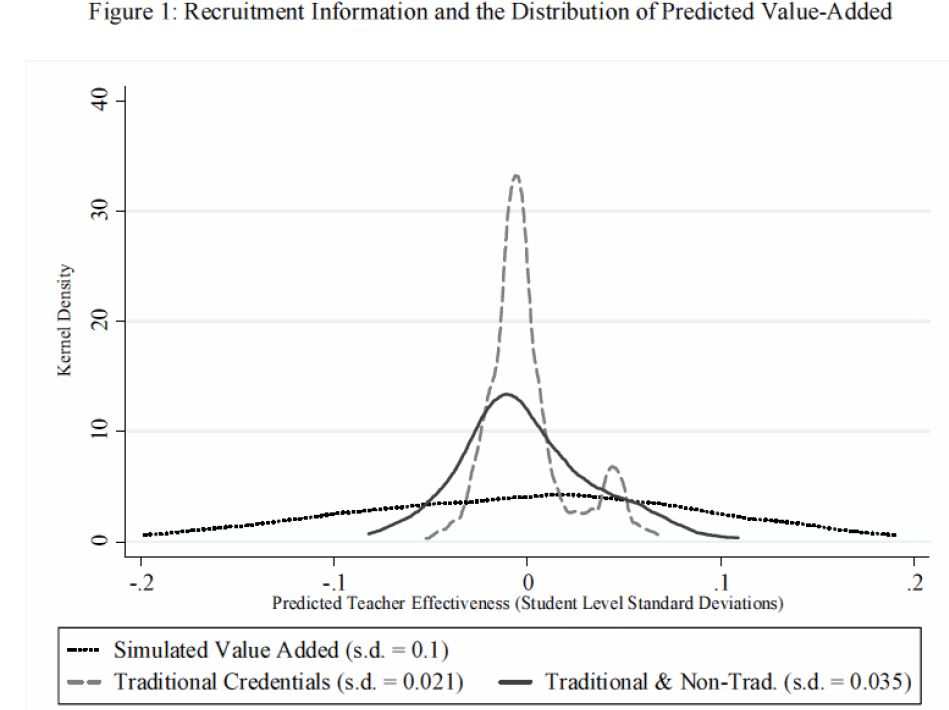
\includegraphics[width=4in]{images/ch9/9 rockoff 5.png}
                \caption{Recruitment Information and the Distribution of Predicted Value-Added}
            \end{figure}

    \subsection{Jacob and Lefgren 2005: Principals' Perceptions?}

        \cite{jacob_principals_2005} alayse whether pricipals can identify good teachers.

        They conclude that subjective principal assessments predict teacher value-added much better than teacher experience, education, and earnings. \empha{Principals are good at identifying the best and the worst teachers, but have trouble distinguishing between teachers in the middle of the distribution.}

\section{Long-Term Impacts of Teachers}

    \subsection{Low Persistence of Teacher Effects and "Teaching to the Test"}

        \cite{jacob_persistence_2008} conclude that teacher value-added in reading and math \emph{quickly erodes}. One year persistence is only around 20\%.

        \cite{carrell_does_2008} explore the random assignment of students to teacher at USAF academy. They find that some teachers get high value-added by "teaching to the test," in order to get better teaching evaluations. The problem is that, by "teaching to the test," they do not teach deep concepts, resulting in low future value-added. Hence, \empha{teachers with low current value-added could have high future value-added}.

    \subsection{2 Studies on Long-Term Impacts of Teachers}

        \subsubsection{\cite{chetty_how_2011}}

            Chetty. Friedman, Hilger, Saez, Schanzenbach, Yagan 2011 investigated the STAR Experiment in which 11571 students in Tennessee were randomly assigned to classrooms within their schools from K-3. Originally, STAR was designed as a class size experiment, but it could be used more generally as a classroom experiment that randomly assign students into good and bad classes (measured by end of class test scores of students in that class).

            Then, Chetty et al. linked STAR records with tax records.
            \begin{figure}[H]
                \centering
                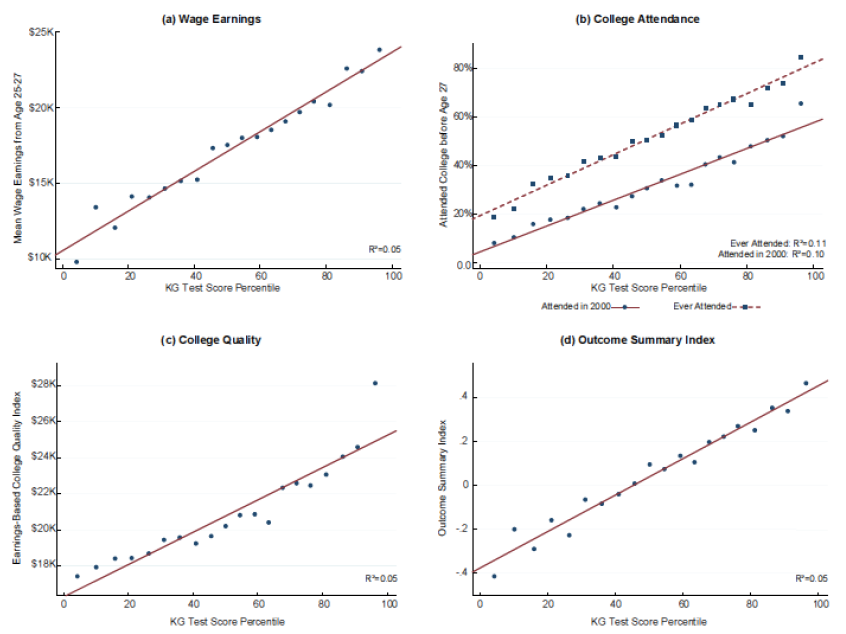
\includegraphics[width=4.5in]{images/ch9/9 chetty 2011 1.png}
                \caption{Scores and Adult Outcomes}
            \end{figure}
            Individual test scores are correlated with adult outcomes.
            \begin{figure}[H]
                \centering
                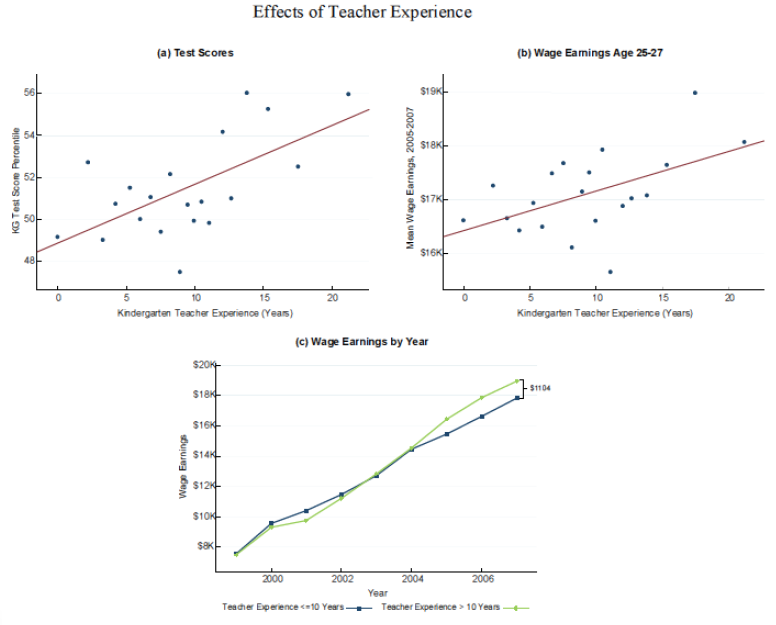
\includegraphics[width=4.5in]{images/ch9/9 chetty 2011 2.png}
                \caption{Effects of Teacher Experience}
            \end{figure}
            Teachers' experience is also correlated with adult outcomes.
            \begin{figure}[H]
                \centering
                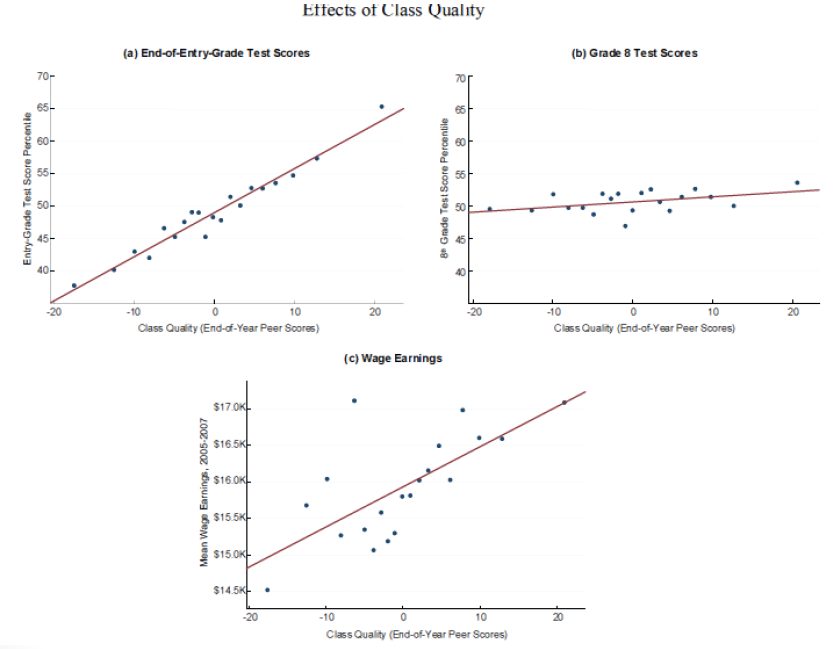
\includegraphics[width=4.5in]{images/ch9/9 chetty 2011 3.png}
                \caption{Effects of Class Quality}
            \end{figure}
            Class quality is also correlated with adult outcomes.
            \begin{figure}[H]
                 \centering
                 \begin{subfigure}[b]{0.4\textwidth}
                     \centering
                     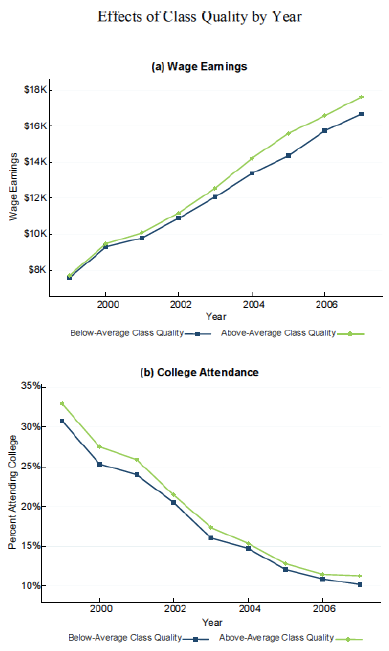
\includegraphics[width=\textwidth]{images/ch9/9 chetty 2011 4.png}
                 \end{subfigure}
                 \begin{subfigure}[b]{0.4\textwidth}
                     \centering
                     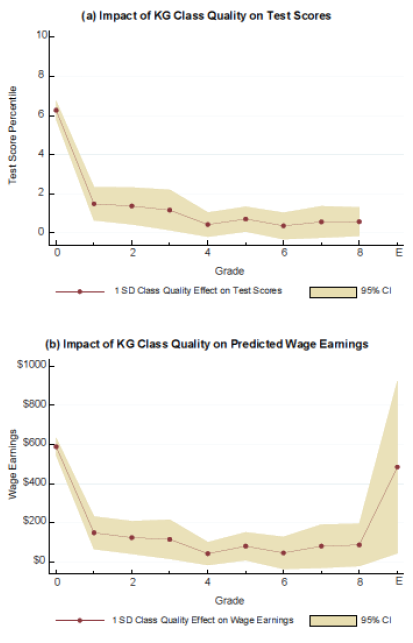
\includegraphics[width=\textwidth]{images/ch9/9 chetty 2011 5.png}
                 \end{subfigure}
                 \caption{Effect of Class Quality by Year}
            \end{figure}
            Effect of class quality on test scores diminish as time goes by, but effects on earnings suddenly appear after some years.

        \subsubsection{\cite{chetty_measuring_2014}}

            Chetty, Friedman, and Rockoff 2014 estimate teacher VA from administrative school records. Specifically, they link VA of teachers assigned to each student to students' tax records. It turns out that distinguishing by grade is not very important.
            \begin{figure}[H]
                \centering
                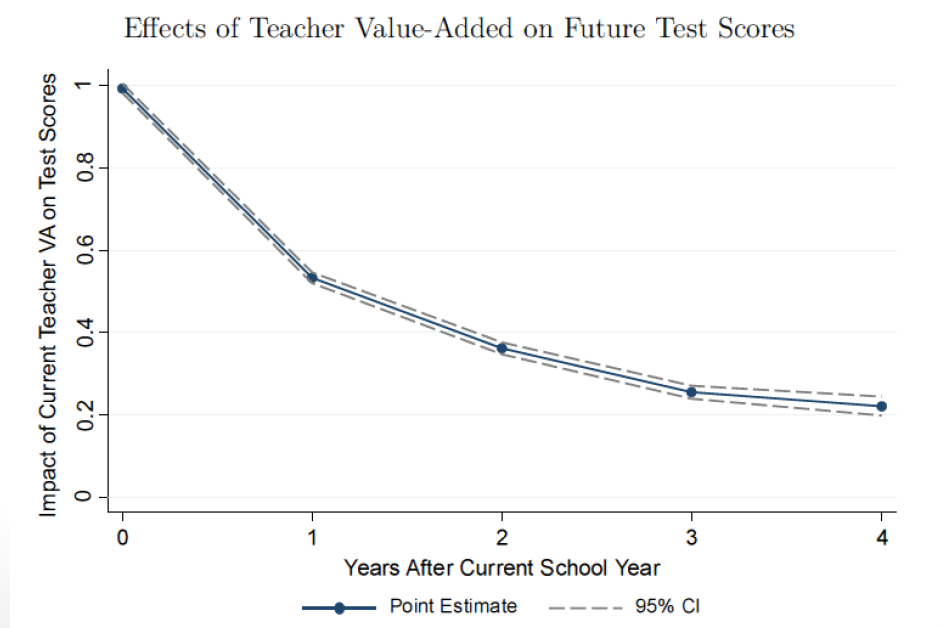
\includegraphics[width=3.5in]{images/ch9/9 chetty 2014 4.png}
                \caption{Teacher VA and Test Scores}
            \end{figure}
            The effect of teacher VA on test score quickly diminishes as age increases.
            \begin{figure}[H]
                \centering
                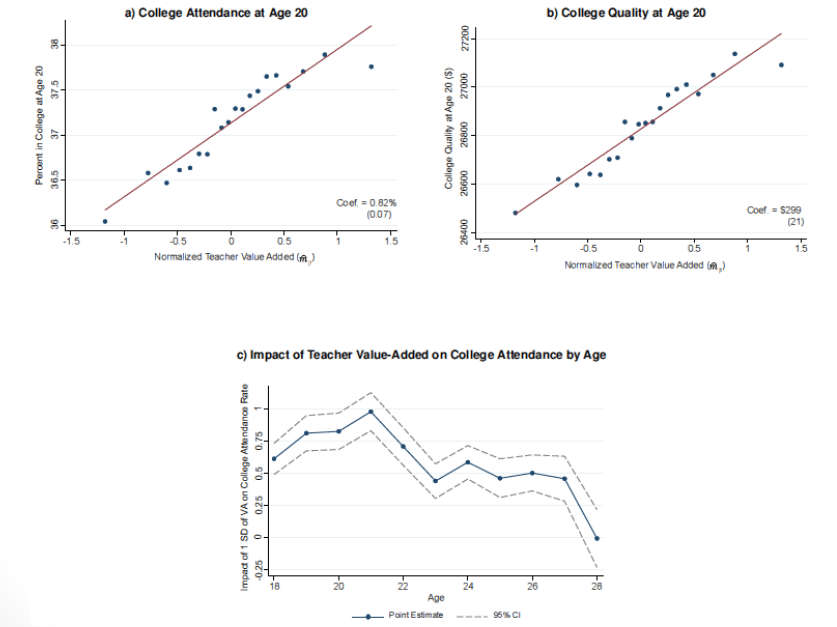
\includegraphics[width=4.5in]{images/ch9/9 chetty 2014 1.png}
                \caption{Teacher VA and College Outcomes by Age}
            \end{figure}
            The effect of teacher VA on college attendance also diminishes.
            \begin{figure}[H]
                \centering
                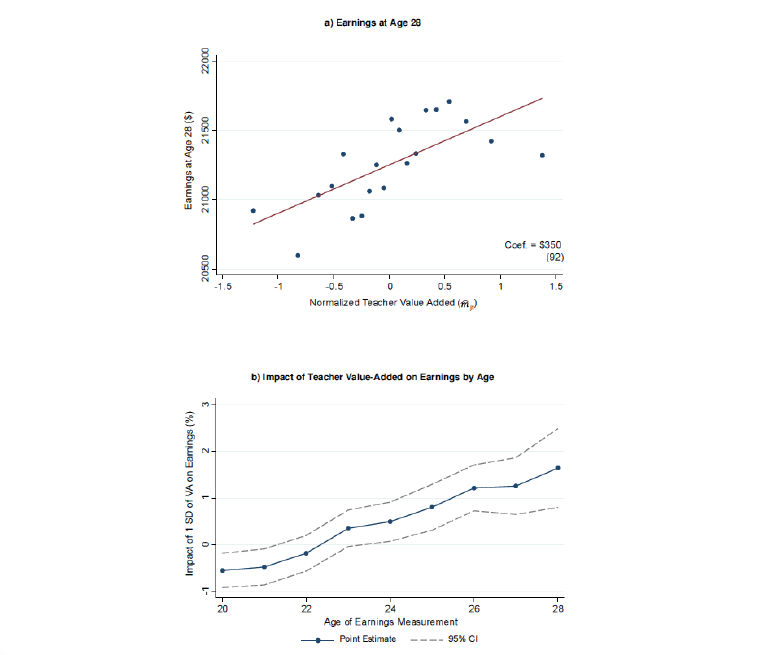
\includegraphics[width=4.5in]{images/ch9/9 chetty 2014 2.png}
                \caption{Teacher VA and Earnings by Age}
            \end{figure}
            However, its effects on earnings increase by time.
            \begin{figure}[H]
                \centering
                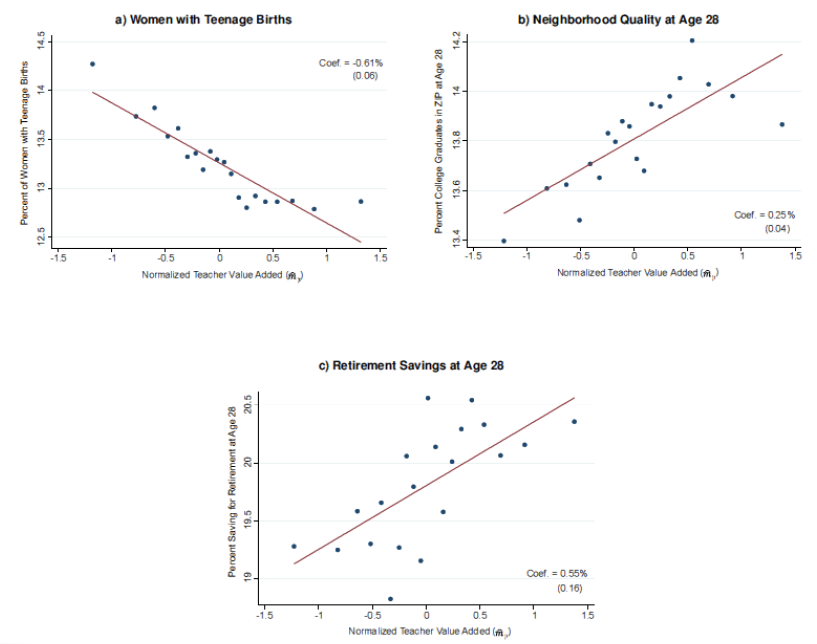
\includegraphics[width=4.5in]{images/ch9/9 chetty 2014 3.png}
                \caption{Teacher VA and Other Adult Outcomes}
            \end{figure}
            Teacher VA is also related to many other adult outcomes.

        \subsubsection{Conclusions}

            A lot of literature, including the above two, found that \empha{effects of teachers on test scores diminish quickly, but their effects on adult outcomes, such as wages, appear and increase after certain time periods.}


    \section{In Developing Countries}

        \cite{araujo_teacher_2016} (Araujo, Carneiro, Cruz, Schady 2016) did a similar study in Ecuador.

        Specifically, they randomly assign kindergarden students to classrooms in schools in Ecuador. They have data from multiple years, so it is possible to distinguish teacher and classroom effects. 

        They test students on multiple dimensions, including Maths, language, executive function, etc. Also, they measure multiple attributes of teachers, including IQ, personality, education, experience, and classroom observations (quality of interaction between teacher and students).
        
        \begin{figure}[H]
            \centering
            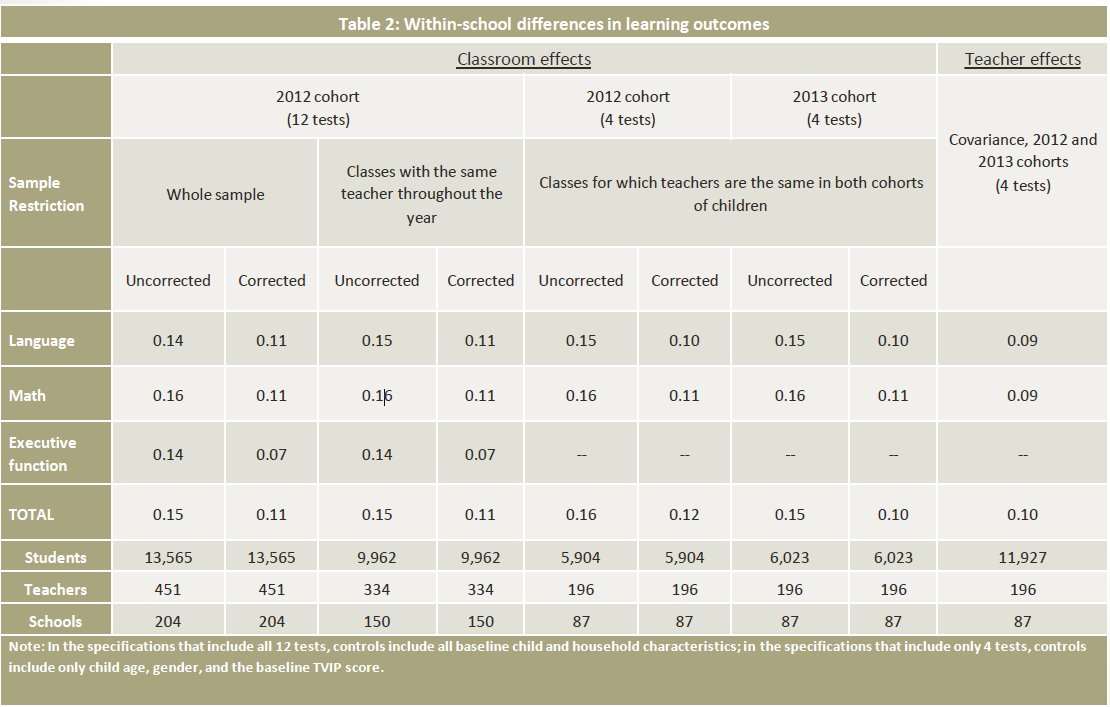
\includegraphics[width=4.5in]{images/ch9/9 Araujo 1.png}
            \caption{With-in School Differences in Learning Outcomes}
        \end{figure}
        \begin{figure}[H]
            \centering
            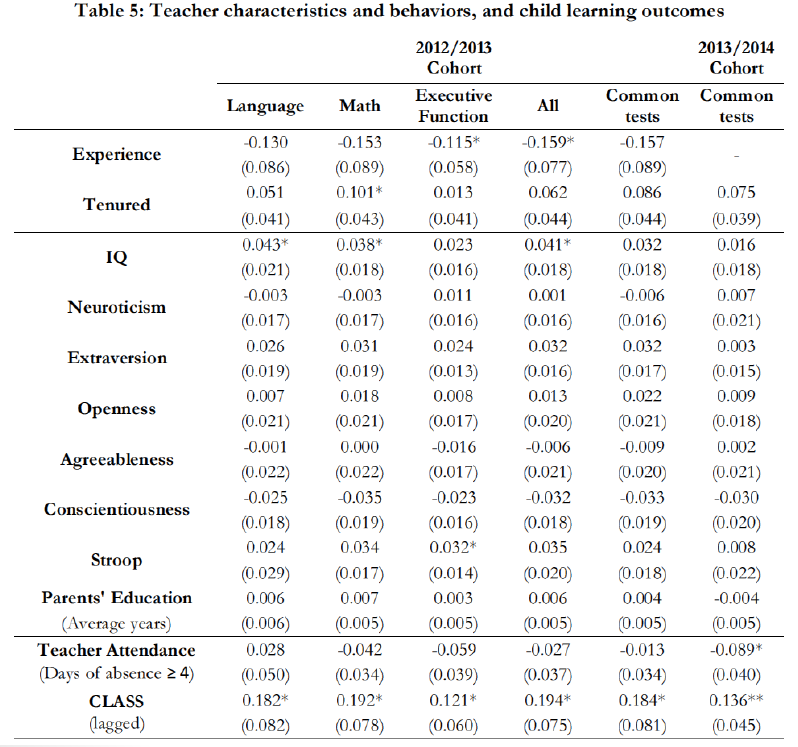
\includegraphics[width=4.5in]{images/ch9/9 Araujo 2.png}
            \caption{Teacher Characteristics \& Behaviours and Child Learning Outcomes}
        \end{figure}
        Still, there's no large and significant characteristics that can be used to predict VA of a teacher.
        \begin{figure}[H]
            \centering
            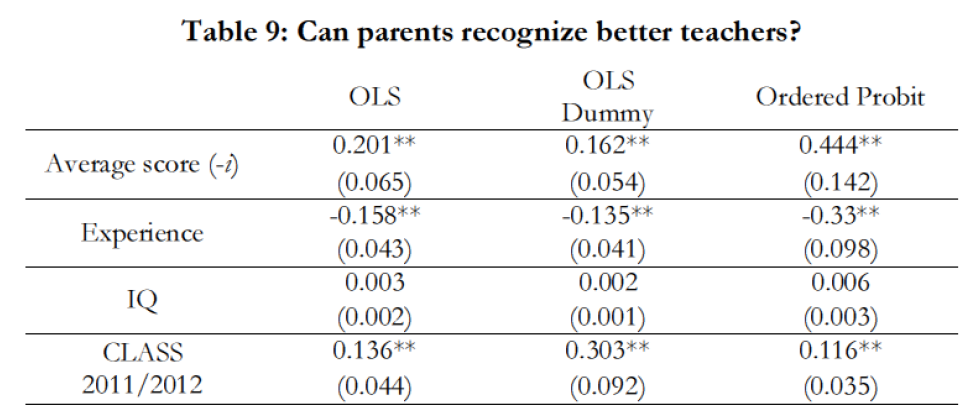
\includegraphics[width=4.5in]{images/ch9/9 Araujo 3.png}
            \caption{Teacher VA and Earnings by Age}
        \end{figure}
        However, parents are able to distinguish good teachers.
        \begin{figure}[H]
            \centering
            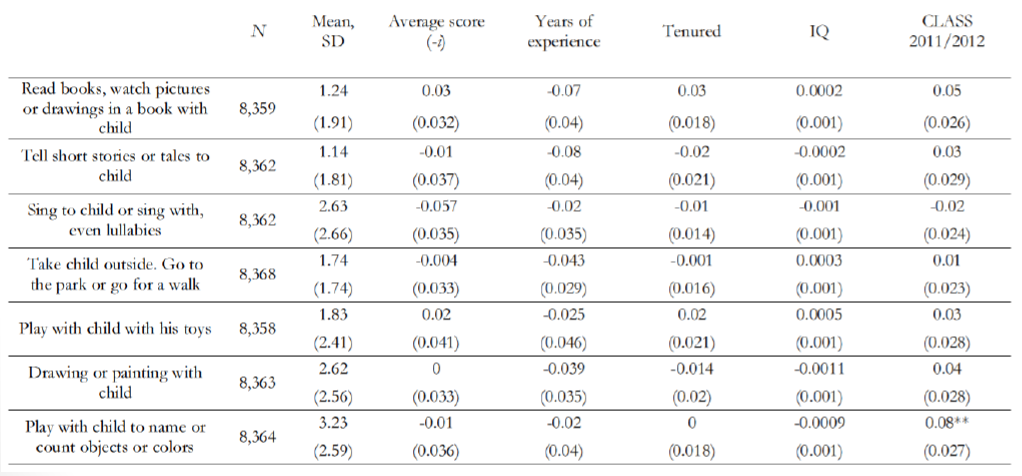
\includegraphics[width=4.5in]{images/ch9/9 Araujo 4.png}
            \caption{Teacher VA and Earnings by Age}
        \end{figure}
        Meanwhile, parents did not seem to respond to teachers' quality.